\chapter{Experiments}
\label{chap:experim}
%\section{Overview}
In this chapter will be shown all the experiments performed and their results. The first section starts from what we expect to show from different code tests and, to this aim, what kind of comparisons will be made.\\
The second section, for each kernel implementation, will explain how tests are set up, ie chosen datasets for each type of code and scripts main features and what results we get. In particular, will be shown time measures and plots with some remarks.
The last section gives a brief summary and some final consideration. Furthermore we'll show comparisons between stream parallel and data parallel version, for each kernel type.

%\section{What and How}
%What and How
\section{Expectations}
As previously mentioned, what we want to see is that our model and implementation for Farm parallel pattern can fit in a GPU.
To this aim is necessary to gain a speedup in the order of the number of Streaming multiprocessors of the GPU we're running code.
Let's clarify some concepts in the sentence above:

\begin{itemize}
	\item The speedup will be estimated in terms of \textbf{GPU completion time}, ie the total time needed to perform all data transfers and kernel executions for a certain application;
	\item We expect to have the best speedup only when we have certain conditions;
	\item The best speedup for would be in the order of multiprocessors number.
\end{itemize}
The last point means we can't expect to reach greater gain than the available amount of hardware resources.\\
Further and specific definitions about these concepts will be given in \hyperref[subs:speedup]{Speedup subsection}.
%This is strictly related to the fact that we can't expect Streaming parallel problems, that we implemented, to perform better than the equivalent Data Parallel version. \footnote{As we mentioned in previous Chapters, the GPU is specifically designed to be efficient and to perform at its best on Data Parallel problems.}
The second point above means we can expect best performances in the following cases:
\begin{itemize}
	\item When we have a regular kernel, that is a kernel with the lowest possible amount of branching and, thus, very low (or absent) threads divergence;
	\item When the kernel is more computational-bound than memory bound, the less access to Global memory the less data transfer latency will slow down execution and this may generally lead to bad occupancy;
	\item When the kernel execution takes an amount of time near the one for data transfer and/or other kernel calls.
\end{itemize} 
When one, or more, of the above conditions isn't met, we expect to have a considerably lower speedup.


\subsection{Measures: What and How}
Before the test setup and writing, it's important to understand what we should measure, in order to get significant comparisons.\\
First we recall that the measures of interest are relative to \textit{data transfers} and \textit{kernel execution} and all completion times are reported in \textbf{milliseconds}. 

In the case were CUDA streams are used, we have an additional time cost to create and destroy streams, especially when lot of streams are spawned.\\
If we want to have as many CUDA Stream as many SMs in device, then creation costs in the order of hundreds of milliseconds and destruction in the order of hundred of microseconds\footnote{Measures on CUDA Streams spawn/deletion were collected with \textit{nvprof} log file, where all CUDA APIs time is precisely measured.}. However, we won't sum them up with measures on data transfer and kernel execution. This is because, even if the streams overhead can be notable, it's a one-time cost to pay.\\
This means that it won't weigh on performances, given that initially we create CUDA streams, then we'll run kernels on a indefinitely long input stream (theoretically) and, only when input is totally consumed out, CUDA streams will be destroyed. 
So on a reasonably long input stream, the CUDA streams APIs cost should be negligible.\\

So focusing on data transfers and kernels, we put two time probes, one before the start of the input stream loop and one at the end. The time probes are implemented using \textbf{CUDA Events}.\\
Below will be reported a pseudo-code to clarify how the probes are placed inside the code:
\begin{lstlisting}[label={lst:timers}]	
/**** Code with events time probes ****/	
streamCreate(streams, nStreams); // Create CUDA streams

createAndStartEvent(&startEvent, &stopEvent); // Create "start" and "stop" events, start recording

int k = 0;
while (InputStream) {  
	if (buffer x[i: i+chunkSize] is full)
	{
		int i = k%nStreams;
		
		kernelCaller(input_host, output_host, input_device, output_device, streams[i], streamBytes, ...);

		. . . .
		
		++k;
	}
	else
	{
		add item to buffer x[i: i+chunkSize]
	}	
} 
msTot = endEvent(&startEvent, &stopEvent);
cudaEventDestroy();
		
/**** Events Creation and start ****/
void createAndStartEvent(cudaEvent_t *startEvent, cudaEvent_t *stopEvent)
{
	gpuErrchk( cudaEventCreate(startEvent) );
	gpuErrchk( cudaEventCreate(stopEvent) );
	gpuErrchk( cudaEventRecord(*startEvent,0) );
}

/**** Events end and time measure collection ****/
float endEvent(cudaEvent_t *startEvent, cudaEvent_t *stopEvent)
{
	float ms = 0.0f;
	gpuErrchk( cudaEventRecord(*stopEvent, 0) );
	gpuErrchk( cudaEventSynchronize(*stopEvent) );
	gpuErrchk( cudaEventElapsedTime(&ms, *startEvent, *stopEvent) );
	return ms;
}
	
/**** Kernel caller example ****/
void kernelCaller(input_host, output_host, input_device, output_device, streams[i], streamBytes, ...)
{
	// H2D mem copy 
	gpuErrchk( cudaMemcpyAsync(input_device, input_host, streamBytes, cudaMemcpyHostToDevice, streams[i]) ); 
	// Kernel call
	ernel<<<GRID, BLOCK, 0, streams[i]>>>(input_device, output_device, ...); 
	#ifndef MEASURES
	gpuErrchk( cudaPeekAtLastError() );
	#endif   
	// D2H mem copy 
	gpuErrchk( cudaMemcpyAsync( output_host, output_device, streamBytes, cudaMemcpyDeviceToHost, streams[i]) );
}
	
\end{lstlisting}
CUDA event APIs are a device-bound tool and they were chosen as inside-code measurement for several reasons.
Another approach could be to use any CPU timer provided for C++ in a way such as:
\begin{lstlisting}
	t1 = myCPUTimer();
	Kernel<<<GRID, BLOCK>>>(param0. param1, ...);
	cudaDeviceSynchronize();
	t2 = myCPUTimer();
\end{lstlisting}
A problem with using host-device synchronization points, such as \texttt{cudaDeviceSynchronize()}, is that they stall the GPU pipeline.
Events, instead, provide a relatively light-weight \footnote{CUDA events make use of the concept of CUDA streams.} alternative to CPU timers via the \textit{CUDA event API}. This API includes calls to create and destroy events, record events, and compute the elapsed time in milliseconds between two recorded events, exactly as it's shown in code Listing \ref{lst:timers}.
 
CUDA events are of type \texttt{cudaEvent\_t} and are created and destroyed with \texttt{cudaEventCreate()} and \texttt{cudaEventDestroy()}. In the above code \texttt{cudaEventRecord()} places the start and stop events into the default stream, or \texttt{stream 0} (also called the “\textit{Null Stream}”). This holds for all device timers we introduced in our code.\\
The \texttt{cudaEventRecord()} will record a time stamp in device for the event, but only when that event is reached in the specified stream. The function \texttt{cudaEventSynchronize()} blocks CPU execution until the specified event is recorded.\\
The \texttt{cudaEventElapsedTime()} function returns the number of milliseconds elapsed between the recording of \textit{start} and \textit{stop}. This value has a resolution of approximately 0.5 microseconds \cite{devblogevents}. So those timers will be enough accurate for our purpose, since we'll see that almost all elapsed times will be from tens to thousands milliseconds.

It's important to point out why we used events on the default streams. 
%If one of the events were last recorded in a non-NULL stream, the resulting time may be greater than expected (even if both used the same stream handle). This happens because the \texttt{cudaEventRecord()} operation takes place asynchronously and there is no guarantee that the measured latency is actually just between the two events.\\
%Any number of other different stream operations could execute in between the two measured events, thus altering the timing in a significant way \cite{libevents}.
Given the asynchronous nature of CUDA calls, that we perform in non-default stream, the behavior and order in between different streams is unpredictable. This means that a call from a different non-null stream can actually be issued in between two events we're trying to recording, even if they were issued from the same non-default stream.\\
This is one of the reasons why we chose to put timers outside the loop over input stream.
We could insert events inside the loop, instead, in that way we'd have measured singularly each iteration\footnote{And so measure each single memory copy H2D, Kernel execution and memory copy D2H.} and sum up all those elapsed times.
There would have been three problems with that approach:
\begin{itemize}
	\item Each "\textit{end}" event, must be sure to measure everything until the ending event, that's why it's necessary to introduce \texttt{cudaEventSynchronize()};
	\item Given that the input stream should be quite long, all those timers in each loop iteration would have introduced an amount of undesired sampling overhead, apart from synchronization time.
\end{itemize}

For first problem, we recall that \texttt{cudaEventSynchronize()} blocks CPU execution until the specified event is recorded, but we really want to avoid that.
We should avoid as much (explicit) host-device synchronizations as we can: given that we're working on input/output streams of items from host, "stopping" this flow on host side at each iteration would invalidate the gain of our model, increasing the overall completion time (probably for a non negligible amount).\\
The second problem is related to the first. Even if events are a light-weight solution for device activities timing, it doesn't mean they don't introduce a bit of overhead (in addition to the synchronization one) in both host and device side.

For completeness, we'll show some performances case of interest measured by profilers, in addition to those from timers.
In designing and implementation phase, this allowed us, not only to observe the correctness of some measurements, but also to check some special cases and their relative technical details and performance analysis.


\subsection{Tests setup}
Once we determined the time measure criterion, we had to decide what behaviors we wanted to observe from our code.% and its performances.
Note that for each type of input dataset, we run multiple times (more precisely 5 times) the executable so that, for a certain input setup, we can collect several time measures. This allows us to delete some \textit{outliers} completion times, as they may distort the result, and then we take the mean value among the remaining measures.

Moreover, as we mentioned in \hyperref[subs:bash]{Subsection 2.5.1}, we implemented our tests as bash scripts.
These scripts will cover the task of:
\begin{itemize}
	\item Compiling a certain executable, exploiting the rules available in our  Makefile;
	\item Run that executable \(N_{test} - 1\) times and then redirect the output, of the running application, to a specific \texttt{.txt} file;
	\item Run for the \(N_{test}^{\ th}\) time the executable via \texttt{nvprof}, redirecting the profiler output to a folder of \texttt{.txt} log files
\end{itemize} 
In next sections we'll show, for each type of kernel, what type of tests have been made and relative results.

It's important to recall that input stream length shouldn't be known a priori, but in tests we'll see that we have to give an input a limit. This is for time measuring purpose only, because we need to have a knowledge on what and how much data we are measuring.


\subsection{Speedup}
\label{subs:speedup}
%Two important metrics related to performance and parallelism are \textbf{speedup} and \textbf{efficiency}. 
An important metric related to performance and parallelism is \textbf{speedup}, it compares the latency for solving a certain computational problem on one hardware unit, generally referred to as \textit{worker}, versus solving the same problem on P hardware units, as below
\begin{center}
	\(speedup = S_{P} = \frac{T_{1}}{T_{P}} \)
\end{center}


where \(T_{1}\) is the latency of the program with one worker and \(T_{P}\) is the latency on P workers.
%\textbf{Efficiency} is speedup divided by the number of workers:
%\begin{center}
%\(efficiency = \frac{S_{P}}{P} =  \frac{T_{1}}{P \cdot T_{P}}\)
%\end{center}
%Efficiency measures return on hardware investment. Ideal efficiency is 1 (often reported as 100\%), which corresponds to a linear speedup, but many factors can reduce efficiency below the ideal.\\
If \(T_{1}\) is the latency of the parallel program running with a single worker, the above equation for speedups, is sometimes called \textit{relative speedup}, because it shows relative improvement from using P workers. This uses a serialization of the parallel algorithm as the baseline. 
Sometimes there is a better serial algorithm that does not parallelize well. \\
If so, it is fairer to use that algorithm for \(T_{1}\), and report \textit{absolute speedup}, as long as both algorithms are solving an identical computational problem. 

An algorithm that runs P times faster on P processors is said to exhibit \textbf{linear speedup}. It is rare in practice, since there is extra work, involved in distributing work to processors and coordinating them. This extra work clearly introduces extra time, also known as \textbf{overhead}.\\
However, as exceptions, an occasional program will exhibit \textbf{superlinear speedup}\footnote{In general, some causes of superlinear speedup may be: restructuring a program for parallel execution can cause it to use memory better (cache in CPU implementations), even with a single worker; or the parallel algorithm  may be able to avoid work that its serialization would be forced to do.}.%, that means an efficiency greater than 100\%. 
However, in general, \textbf{sublinear speedup} is the norm\cite{structparprog}.

\textbf{Amdahl's Law} gives an important limit on speedup: it considers speedup as P varies and the problem size remains fixed.\\
Amdahl identified in the execution time \(T_{1}\) of a program, two categories: time spent doing \textit{non-parallelizable serial work} and time spent doing \textit{parallelizable work}. Call these \(T_{ser}\) and \(T_{par}\) , respectively. \\
Given P workers available to do the parallelizable work, the times for sequential and parallel execution are:
\begin{center}
	\(T_{1} = T_{ser} + T_{par}\) \\
	\(T_{P} \geq T_{ser} + \frac{T_{par}}{P}\)
\end{center}

The bound on \(T_{P}\) assumes no superlinear speedup, and is an exact equality only if the parallelizable work can be perfectly parallelized.\\
Plugging these relations into the definition of speedup, we gave before, yields \textbf{Amdahl’s Law}:
\begin{center}
	\(S_{P} \leq \frac{T_{ser}+T_{par}}{T_{ser}+T_{par}/P}\)
\end{center}
%Amdahl’s Law has an important corollary. 
Let \(f\) be the non-parallelizable serial fraction of the total work. Then the following equalities hold:
\begin{center}
	\(T_{ser} = f \cdot T_{1}\)\\
	 \(T_{par} = (1-f) \cdot T_{1}\)
\end{center}

Substituting these into speedup equation:
\begin{center}
	\(S_{P} \leq \frac{1}{f+(1-f)/P}\  \Rightarrow \  S_{\infty} \leq \frac{1}{f}\)
\end{center}

Speedup is \textit{limited by the fraction of the work that is not parallelizable}, even using an infinite number of processors\cite{structparprog}.\\
%For example if 10\% of the application cannot be parallelized, then the maximum speedup is 10x.
%If 1\% of the application cannot be parallelized, then the maximum speedup is 100x.\\
%In practice, an infinite number of processors is not available. With fewer processors, the speedup may be reduced, so the equation above gives an upper bound on the speedup.

%This limitation on speedup can also be viewed as inefficient use of parallel hardware resources for large serial fractions, as shown in Figure 2.6.

%Amdahl's Law views programs as fixed and the computer as changeable, but experience indicates that as computers get new capabilities, applications change to exploit these features.\\

%Gustafson noted that problem sizes grow as computers become more powerful. As the problem size grows, the work required for the \textit{parallel part of the problem frequently grows much faster than the serial}.\\
%If this is true for a given application, then, as the problem size grows, the serial fraction decreases and speedup improves.
%Suppose that the serial portion is constant while the parallel portion grows linearly with the problem size. As workers are added, the application solves bigger problems in the same time, or the same problem in less time.\\
%The serial portion still takes the same amount of time to perform, but diminishes as a fraction of the whole. Once the serial portion becomes insignificant, speedup grows practically at the same rate as the number of processors, thus achieving linear speedup.

%Both Amdahl's and Gustafson-Barsis' Laws are correct. The difference lies in whether we want to make a program run faster with the same workload or run in the same time with a larger workload.\\

%Furthermore, Gustafson-Barsis’ observation is not a license for carelessness. In order for it to hold it is critical to ensure that serial work grows much more slowly than parallel work, and that synchronization and other forms of overhead are scalable.


%2.5.6 Work-Span Model
%This section introduces the work-span model for parallel computation. The work-span model is much more useful than Amdahl’s law for estimating program running times, because it takes into account imperfect parallelization. \\
%Furthermore, it is not just an upper bound as it also provides a lower bound.
%It allows to estimate \(T_{P}\) from just two numbers: \(T_{1}\) and \(T_{\infty}\).

%In the work-span model, tasks form a directed acyclic graph. A task is ready to run if all of its predecessors in the graph are done. 
%The basic work-span model ignores communication and memory access costs. It also assumes task scheduling is greedy, which means the scheduler never lets a hardware worker sit idle while there is a task ready to run.

%The extreme times for\(P=1\) and \(P=\infty\) are most important.\\
%Time \(T_{1}\) is called the \textbf{work} of an algorithm. It is the time that a serialization of the algorithm would take and is simply the total time it would take to complete all tasks.\\
%Time \(T_{\infty}\) is called the \textbf{span} of an algorithm. The span is the time a parallel algorithm would take on an ideal machine with an infinite number of processors.

%Span is equivalent to the length of the critical path. The critical path is the longest chain of tasks that must be executed one after each other. 

%Work and span each put a limit on speedup.\\ Superlinear speedup is impossible in the work-span model:
%\begin{center}
%	\(S_{P} = \frac{T_{1}}{T_{P}} \leq \frac{T_{1}}{T_{1}/P} = P\)
%\end{center}
%On an ideal machine with greedy scheduling, adding processors never slows down an algorithm:
%\begin{center}
%	\(S_{P} = \frac{T_{1}}{T_{P}} \leq \frac{T_{1}}{T_{\infty}}\)
%\end{center}
%In words:
%\begin{center}
%	\(speedup = \frac{work}{span}\)
%\end{center}
%Real machines introduce synchronization overhead, not only for the synchronization constructs themselves, but also for communication. A span that includes these overheads is called a \textbf{burdened span}.

%The span can also be used to estimate a lower bound on speedup for an ideal machine. An inequality known as Brent's Lemma bounds \(T_{P}\) in terms of the work \(T_{1}\) and the span \(T_{\infty}\):
%\begin{center}
%	\(T_{P} = \frac{T_{1}-T_{\infty}}{P+T_{\infty}}\)
%\end{center}
%Here is the argument behind the lemma. The total work \(T_{1}\) can be divided into two categories:
%perfectly parallelizable work and imperfectly parallelizable work. The \textit{imperfectly parallelizable work} takes time \(T_{\infty}\), no matter how many workers there are.\\
%The \textit{perfectly parallelizable work} remaining takes time \(T_{1}-T_{\infty}\) with a single worker, and since it is perfectly parallelizable it speeds up by P if all P workers are working on it. 
%But if not all P workers are working on it, then at least one worker is working on the \(T_{\infty}\) component. The argument resembles Amdahl’s argument, but generalizes the notion of an inherently serial portion of work to imperfectly parallelizable work.
%Though the argument resembles Amdahl's argument, it proves something quite different. Amdahl's argument put a lower bound on \(T_{P}\) and is exact only if the parallelizable portion of a program is perfectly parallelizable. Brent's Lemma puts an upper bound on \(T_{P}\). It says what happens if the worst possible assignment of tasks to workers is chosen.
%In general, work-span analysis is a far better guide than Amdahl’s Law, because it usually provides
%a tighter upper bound and also provides a lower bound. Figure 2.9 compares the bounds given by
%Amdahl’s Law and work-span analysis for the task graph in Figure 2.8. There are 18 tasks. The first
%and last tasks constitute serial work; the other tasks constitute parallelizable work. Hence, the fraction
%of serial work is 2/18 = 1/9. By Amdahl’s Law, the limit on speedup is 9. Work-span analysis says the
%speedup is limited by the min(P, T 1 /T ∞ ) = min(P, 18/6), which is at most 3, a third of what Amdahl’s
%law indicates. The difference is that the work-span analysis accounted for how parallelizable the parallel work really is. The bottom curve in the figure is the lower bound provided by Brent’s lemma.
%It says, for example, that with 4 workers a speedup of 2 is guaranteed, no matter how the tasks are assigned to workers.
%Brent’s Lemma leads to a useful formula for estimating T P from the work T 1 and span T ∞ . To get much speedup, T 1 must be significantly larger than T ∞ , In this case, T 1 − T ∞ ≈ T 1 and the right side of 2.8 also turns out to be a good lower bound estimate on T P . So the following approximation works well in practice for estimating running time:
%T P ≈ T 1 /P + T ∞ if T ∞
%T 1 .


%The approximation says a lot:
%-Increasing the total work T 1 hurts parallel execution proportionately.
%-The span T ∞ impacts scalability, even when P is finite.
%When designing a parallel algorithm, avoid creating significantly more work for the sake of parallelization, and focus on reducing the span, because the span is the fundamental asymptotic limit on scalability. Increase the work only if it enables a drastic decrease in span. An example of this is the scan pattern, where the span can be reduced from linear to logarithmic complexity by doubling the work (Section 8.11).
%Brent’s Lemma also leads to a formal motivation for overdecomposition. From Equation 2.8 the following condition can be derived:
%S P = T 1 /T P ≈ P if T 1 /T ∞
%P.

%It says that greedy scheduling achieves linear speedup if a problem is overdecomposed to create much
%more potential parallelism than the hardware can use. The excess parallelism is called the parallel
%slack, and is defined by:
%parallel slack =
%S ∞
%T 1
%=
%P
%PT ∞
%(2.11)
%In practice, a parallel slack of at least 8 works well.
%If you remember only one thing about time estimates for parallel programs, remember Equation 2.9.
%From it, you can derive performance estimates just by knowing the work T 1 and span T ∞ of an
%algorithm. However, this formula assumes the following three important qualifications:
%-Memory bandwidth is not a limiting resource.
%-There is no speculative work. In other words, the parallel code is doing T 1 total work, period.
%-The scheduler is greedy.
%The task schedulers in Intel Cilk Plus and Intel TBB are close enough to greedy that you can use the approximation as long as you avoid locks. Locks make scheduling non-greedy, because a worker can get stuck waiting to acquire a contended lock while there is other work to do. Making performance predictable by Equation 2.9 is another good reason to avoid locks. Another trait that can make a scheduler non-greedy is requiring that certain tasks run on certain cores. In a greedy scheduler, if a core is free it should immediately be able to start work on any available task.


\subsection{Results: gathering and evaluation}
\label{subs:resgath}
From all \texttt{.txt} files, containing time measures for all the execution that have been run from tests, we have to work on some results and calculations.\\
In particular, implemented Python scripts \footnote{See \hyperref[chap:tools]{Chapter 2}.} provides a tool to:
\begin{itemize}
	\item First of all, output all necessary \texttt{.csv} containing all averages, of the times got by the multiple runs for a certain input \footnote{Remember that outliers values are rejected, and mean values are computed on remaining values.};
	\item Then from all those average Completion times, in \texttt{.csv} format, another script computes all \textbf{Speedups};
	\item Finally, the same script that computes speedups, outputs plots on most significant results.\\
\end{itemize}

It's important to point out what kind of speedups will be computed, so that in next sections we can presents numeric and graphic results.\\
Remembering what we introduced in \hyperref[subs:speedup]{Section 5.1.3}, for a certain program, the speedup, in brief, is the ratio between the time spent in sequential (or single worker) version and the time spent on parallel version, having P workers:
\begin{center}
	\(speedup = S_{P} = \frac{T_{1}}{T_{P}} \)
\end{center}
Here we have to define what those times correspond in our implementation:
\begin{itemize}
	\item \(T_{1}\), ie the sequential version, is the case in which CUDA Streams aren't used\footnote{More precisely only default stream is used, instead non-default streams aren't used.}. In a sense, this corresponds to serialize all data transfers and kernel execution as
	\begin{center}
		\(H2D_{0},\ Ker_{0},\ D2H_{0},\ H2D_{1},\ Ker_{1},\ D2H_{1}, . . .\)
	\end{center}
	So, even if we have a stream of item as input, this means sending only a small chunk at time to the device, thus using only a small amount of computational resources at time;
	\item \(T_{P}\), ie parallel version, is the case in which CUDA Streams are used, where P will be the number of non-default streams spawned.
\end{itemize}
In the particular scenario of a Farm for GPU, the number of workers has a more complex meaning. Those workers, more precisely, corresponds to how many Streaming Multiprocessors we're going to use in the GPU, ie the target numbers of SMs we want to make busy at computation peak time.\\
So the speedup, obtained from those two implementations, will also give us an indicator on how many SMs will be effectively used.
In other words, here we can see a CUDA stream as a sort of channel in which we put tasks and we want to see if those channels will successfully overlap, hiding data transfer from/to device, executing multiple kernels at the sametime and other possible latencies.
So, the computed speedups are:
\begin{enumerate}
	\item \(speedup = S_{3} = \frac{T_{1}}{T_{3}} \) as we mentioned before, this is a base case for CUDA streams use;
	\item \(speedup = S_{\#SM} = \frac{T_{1}}{T_{\#SM}} \) this is the special case that aims to make Farm parallel pattern fitting in GPUs architecture.\\
\end{enumerate}

The way we defined speedup lead us to ask what is the best we can achieve and this is where Amdahl's law can be applied.\\
First we should define what are completion times, upon which we base analysis. Suppose we focus on a portion of input/output stream made of \(n\) elements:
\begin{center}
	\(T_{Tot} = n \cdot (T_{In Stream} + T_{H2D} + T_{Kernel} + T_{D2H} +T_{Out Stream}) \)
\end{center}
Below we'll explain this formula's components:
\begin{enumerate}
	\item 	\(T_{Tot}\) is the overall time it takes to compute \(n\) elements from an input stream, ie latency from the first available item on the input stream, until the last result item is sent to the output stream (this involves both host and device elapsed times);
	
	\item 	\(T_{In_Stream}\) this is the time it takes to get a chunk from input stream of size \(k << n\)\footnote{It's a buffer of \(k\) floats in Simple-computational kernel, while it's a matrix of \(k\) items in Matrix Multiplication kernel, or an image with \(k\) pizels} (host measure);
	
	\item 	\(T_{H2D}\) is the time spent in transferring a chunk of \(k\) items from host to device (device time);
	
	\item \(T_{Kernel}\) is the time needed by the GPU to compute a certain kernel on \(k\) elements (device time);
	
	\item 	\(T_{D2H}\) is the time spent in transferring back \(k\)-sized results from device to host (device time);
	
	\item 	\(T_{Out_Stream}\) the time it takes to send results to the output stream (host measure).
\end{enumerate}
Obviously measures and all considerations are based only on device completion times, ie points 3,4 and 5 of the above list.\\
We can reduce our test to an important assumption: we don't know how much it is \(n\) (the real length of the input stream), that's why we focus our measures on a reasonably long portion of the input stream, ie \((l \cdot k) < n\) elements will be the stream limit.\\
So we'll focus our attention exclusively to:
\begin{center}
	\(T_{Device} = l \cdot T_{Comp}\)\\
	where\\
	\(T_{Comp}=k \cdot(T_{H2D} + T_{Kernel} + T_{D2H})\)\\
\end{center}
In other words 	\(T_{Comp}\) is the time needed to send a chunk of \(k)\)
items to GPU, make computations on them and then send back to host  \(k)\) results.\\
As we told before, host elapsed times aren't in the study domain of this thesis. So, what we want to parallelize is \(T_{Device}\), in particular we want all \(l\) chunks to run in parallel. Clearly, we're also assuming that \(l > \#SM\), ie our tests will run on a limited input stream, but still ensuring that we have several tasks to send for each CUDA streams, consequently more tasks per SM.\\
Following all these assumptions, it's normal to ask what would it be the maximum reachable speedup and to define this we exploit Amdahl law, showed in previous section. Recall that according to Amdahl, serial code can be identified in two categories: serial fraction and parallelizable fraction.\\
Since we're only focusing on \(T_{Device}\) and, since we wish to parallelize all of it, ideally all operations included in this completion time may be considered parallelizable. This leads trivially to: \(f=0\) and  \((1-f)=1\).\\
Merging this with the Amdahl's upper bound we obtain:
\begin{center}
		\(S_{P} \leq \frac{1}{f+(1-f)/P}\   = \frac{1}{1/P}=P\)
\end{center}
And since we have a limited amount of resources, given by the Streaming Multiprocessors number, we can conclude that the maximum speedup we can achieve is: \(Sp_{\#SM} \leq \#SM\). This formally proves our expectations.
%\Rightarrow \  S_{\infty} \leq \frac{1}{f}


In the next sections will be reported all completion times and speedups, that are mostly representative. 
For each type ok kernel, that was implemented,  we'll show inputs, tests and results (with some graphics and plots).




%%%%%%%%%%%%%%%%%%%
%%%%% COSINE  %%%%%
%%%%%%%%%%%%%%%%%%%
\section{Simple-computation kernel}
For the computational-bound kernel, for each type of input dataset, we identified three different values of kernel iterations number, call it \(M\), it takes the following values: \(10 000, 400 000, 800 000\).\\
These values identify how many times the kernel will have to repeat a certain mathematical operation (in our case the Cosine).

Another important parameter is the Block size that we set to \(BLOCK = (1024, 1, 1)\). We recall that 1024 is the maximum we can give to \textit{x} and \textit{y} block dimension, this holds for both of the GPUs we used to run tests, ie \textbf{P100} and \textbf{M40}.\\
The choice for 1024 was made according to CUDA Occupancy APIs, that suggested this as best block size for the considered application. In general, but it's not a strict rule, computational-bound kernels perform at their best on higher block size, because this should allow us to use the maximum number of threads possible and, thus, to use as much computational resources as possible.\\
%As we mentioned in \hyperref[chap:logic]{Chapter 3}
%Then, for each iterations amount, we performed the following executions in \hyperref[tab:cosdata]{Table 5.1}, here are reported all limits on input stream length.
	\begin{table}	
		\centering
		\begin{tabular}{| c c |} 
			\hline
			\textbf{Tesla P100} & \textbf{Tesla M40} \\ [0.5ex] 
			\hline\hline
			
			57 344 & 24 576  \\ 
			\hline		
			114 688	& 49 152  \\ 
			\hline			
			229 376 & 98 304 \\
			\hline				
			458 752 & 196 608 \\
			\hline
			917 504 & 393 216 \\
			\hline
			1 835 008 & 786 432 \\
			\hline

		\end{tabular}
		\caption{Input dataset for Simple-Computation kernel, these are the input stream length for both devices.}	
		\label{tab:cosdata}		
	\end{table}

All types of tests performed on Simple-computational kernel are:
\begin{enumerate}
	\item \textbf{Classic data parallel approach}\\
		Here we launch the execution of our simple-computation kernel, as it would be classically used: as data parallel application.\\
		To this aim, we should assume that, instead of having as input a stream of items, we have a quite long array of data, in particular consisting of floating point numbers.\\
		In \hyperref[tab:cosdata]{Table 5.1} we show length that was used, in this case is the number of items grouped in a data structure.\\
		Note that, as in all data parallel versions we implemented, we don't make use of CUDA Streams, they'd be useless since we're launching a single kernel on a single huge data structure.

		
	\item \textbf{Streaming parallel with smaller buffers}
		Here we're facing the Farm parallel pattern for GPU, but with smaller buffers.
		As we mentioned in \hyperref[chap:logic]{Chapter 3}, we're trying to get maximal occupancy, especially in a computational-bound kernel.\\
		So, given that the goal of our code is that each called kernel  could fill fully or partially a SM, we had to take into account of: 
		\begin{itemize}
			\item How many items we push for each kernel execution;
			\item Consequently, how many thread blocks our kernel will issue.
		\end{itemize}
		These choices followed from our devices features, though the two GPUs are located in different Compute Capabilities (P100 is c.c. 6.0, M40 is c.c. 5.2) they have the same limits for 
		\begin{itemize}
			\item Resident \textbf{threads} per SM = 2048 (equivalent to 64 resident warps per SM);
			\item Resident \textbf{thread blocks} per SM = 32.
		\end{itemize}
		The second limit means that we can have at most 32 thread blocks active, and so running, on a certain Streaming Multiprocessor. However we can hit this limit only when we have a poor amount of threads in each block or a consistent quantity of thread blocks.\\
		These aren't our case, since we decided to use the maximum number of threads in a block, ie for \textit{x} block dimension and the lowest possible size in grid.
		
		The first limit, instead, is our main goal here. Having at most 2048 active threads in a SM and having configuration of \texttt{blocks = (1024, 1, 1)}, we will have at most two resident blocks in a SM.
		
		The execution configuration for smaller buffers is such that we want to have 1024 buffers and kernel configuration such as \texttt{<<<1, 1024>>>}. 
		So here each launched kernel will have one block containing 1024 threads and this theoretically should correspond to half the occupancy of a SM.\\
		Clearly the code will launch a lot of buffers to device, ie enough to hopefully fill all SMs. We recall that the number of chunks will be limited according to values in \hyperref[tab:cosdata]{Table 5.1}.
		
		All of the above mentioned configurations will be tested for the following CUDA streams cases:		
		\begin{itemize}
			\item \textbf{Zero} CUDA Streams. This is the scenario where we use any non-default CUDA stream, so we'll have serial and synchronous data transfers. Kernel are still an asynchronous call, but immediately after we want to have data back from device and this means have a \texttt{cudaMemcpy}, ie a synchronous call (w.r.t. the host);
			\item \textbf{Three} CUDA Streams. Here we'll use 3 non-default streams, because we want to observe the behavior of our code in a sort of base case. In general, using three stream is the classic configuration for devices with two copy engines. This means it's the minimum to expect an overlap such as a kernel and at most two simultaneous data transfers;
			\item \textbf{N\textsubscript{SM}} CUDA Streams, with \(N_{SM}\ =\#Streaming \ Multiprocessors\). This is the special case because, in general, applications don't use such a high number of CUDA Streams. But in our case it's necessary to try to achieve the expected speedup with respect to the version without non-default streams (we'll sometimes refer to as "zero version").\\
			Clearly, at a certain time say \(t_{i}\), we can have at most two data transfer but there's no limit on kernel calls, clearly they will be effectively executed as long as there are available resources on the device. So this is the key point why all of kernel launches, at peak CUDA stream filling, should be spread in SMs, as soon as requested resources will be available.
		\end{itemize}
		
	\item \textbf{Streaming parallel with bigger buffers}
	This tests setup has similar premises to the one for smaller buffers, here the only thing is changing is buffer length set to 2048.\\
	Thus, having always \texttt{blockSize=(1024, 1, 1)}, the code will set \texttt{gridSize=(2, 1, 1)}, this is because we'll have two blocks, each covering calculations on one half of the buffer.
	This can sound as having better performances, with respect to smaller buffers, but, as we said before, it's not a strict rule to have better performances on maximum occupancy.
	We'll see from results that instead this approach behaves worse than smaller buffers. \\
	Clearly we repeated the above mentioned amount of CUDA streams, so for this configuration we executed code using: \textbf{Zero}, \textbf{Three} and \textbf{N\textsubscript{SM}} CUDA Streams.
	%Motivations for those number of non-default streams are completely analogous to the one explained before.



	%FUTURE VERSION
	%\item \textbf{Streaming parallel using \texttt{std::future} approach (smaller buffers)}
	%Here's a particular case, because we wanted to experiment a different approach for host side.
	%Until now we have seen all cases in which CUDA calls were issued synchronously by a single host thread, ie the main thread.\\
	%We tried, instead, to see what could happen if we used more threads calling in asynchronous way, at each iteration, a copy H2D, kernel call, and copy D2H.\\
	%We tested only a single scenario, \textbf{N\textsubscript{SM}} CUDA Streams, just to observe, in our CUDA stream special case, if this approach would have give even more advantage, than single thread host.
	
\end{enumerate}
\begin{table}	
	\centering
	\begin{tabular}{ | c ||  c | c  || c | c | } 
		\hline
		&  \multicolumn{2}{c}{\textbf{Tesla P100 (zero stream)}} & \multicolumn{2}{c}{\textbf{Tesla M40 (zero stream)}}\\ [0.5ex]
		% & \textbf{Tesla P100} & \textbf{Tesla M40} \\ 
		\hline
		M iterations & Event Times & N elements    &    Event Times & N elements  \\
		\hline\hline
		
		
		10000 &	4622.86 &	\multirow{3}{*}{57344}&	693.747&	\multirow{3}{*}{24576}\\
		400000 & 181465.333&	&	27453.933&	\\
		800000 &	361199.666&	&	54888.933&	\\
		\hline
		10000 &	9294.18&	\multirow{3}{*}{114688}&	1382.363&	\multirow{3}{*}{49152}\\
		400000 &	281507 &	&	54901.6333&	\\
		800000 &	407750.666&	&	109783.666&	\\
		\hline
		10000 &	10217.933&	\multirow{3}{*}{229376}&	2765.323&	\multirow{3}{*}{98304}\\
		400000 &	407779.666&	&	109799.333&	\\
		800000 &	815513.666&	&	219553&	\\
		\hline
		10000 &	20433.633&	\multirow{3}{*}{458752}&	5528.96&	\multirow{3}{*}{196608}\\
		400000 &	815561&	&	219589&	\\
		800000 &	1631013.333&	&	439097.666&	\\
		\hline
		10000 &	40865.4&	\multirow{3}{*}{917504}&	11058.433&	\multirow{3}{*}{393216}\\
		400000 &	1631096.666&	&	439192.333&	\\
		800000 &	3261986.666&	&	878195&	\\
		\hline
		10000 &	81731.733&	\multirow{3}{*}{1835008}&	22112.6&	\multirow{3}{*}{786432}\\
		400000 &	3262250	& &	878433&	\\
		800000 &	6617950 &	&	1756373.333&	\\
		\hline
	\end{tabular}
	\caption{Device completion times for Simple-computation kernel, without using CUDA Streams, results are reported for both machines (P100 and M40).}	
	\label{tab:cosavgszero}		
\end{table}

\begin{table}	
	\centering
	\begin{tabular}{ | c |  c c  | c c | } 
		\hline
		& \multicolumn{2}{c}{\textbf{Tesla P100 (56 Streams)}} & \multicolumn{2}{c}{\textbf{Tesla M40 (24 Streams)}}\\ [0.5ex]
		% & \textbf{Tesla P100} & \textbf{Tesla M40} \\ 
		\hline
		M iterations & Event Times & N elements    &    Event Times & N elements  \\
		\hline\hline
		
		10000 &	104.772& \multirow{3}{*}{57344}& 30.6074& 24576\\
		400000&	3968.913&	&	1178.72	& 24576\\
		800000&	7818.843&	&	2355.413&	24576\\
		\hline
		10000&	205.729&\multirow{3}{*}{114688}& 60.208& 49152\\
		400000&	7828.193&	&	2358.656&	49152\\
		800000&	15691.833&	&	4714.36&	49152\\
		\hline
		10000&	407.712& \multirow{3}{*}{229376}& 119.3446&	98304\\
		400000&	15687.966&	&	4715.123&	98304\\
		800000&	31396&	&	9425.92&	98304\\
		\hline
		10000&	803.223& \multirow{3}{*}{458752}& 238.249&	196608\\
		400000&	31422.033&	&	9429.89&	196608\\
		800000&	62818.7&	&	18853.966&	196608\\
		\hline
		10000&	1619.586& \multirow{3}{*}{917504}&	475.590&	393216\\
		400000&	62793.4&	&	18856.8&	393216\\
		800000&	125575&	&	37705.666&	393216\\
		\hline
		10000&	3229.063& \multirow{3}{*}{1835008}&	949.497 & 786432\\
		400000&	125547.666&	&	37711.9 &	786432\\
		800000&	251503&	&	75445.266&	786432\\
		
		\hline
	\end{tabular}
	\caption{Device completion times for Simple-computation kernel, using as many CUDA Streams as SM number, results are reported for both machines (P100 and M40).}	
	\label{tab:cosavgsSM}		
\end{table}

\subsection{Results}
All the above tests on Simple-Computation Kernel give us the measures of device times, on which most of observations will rely on.\\
We can group the measures into two parts:\\\\\\
	{\large \textbf{Smaller buffers}}\\
	All collected elapsed times for 1024-long buffers are reported in \hyperref[tab:cosavgszero]{Table 5.2}, for the zero-streams version, and \hyperref[tab:cosavgsSM]{Table 5.3}, for the SM-streams version.\\
	From measures in \hyperref[tab:cosavgszero]{Table 5.2}(zero-streams) we can see that Completion Time, fixed an input stream length, increases proportionally with iterations number (eg completion times for 40 000 iterations kernel compared to the one for 1000, is almost \(40\times\) bigger). This holds on both of devices.\\
	This is a clear sign that this type of kernel is computation-bound.\\
	Furthermore, input stream lengths grows by a factor of 2.\\ 
	Always looking at  \hyperref[tab:cosavgszero]{Table 5.2}, fixed a number of iterations, we can see that even completion times grows by a factor of 2.\\
	Again this confirms that, no matter how many elements the input stream sends, no matter how many iterations the kernel does, \textit{we'll have a completion time directly proportional to the computations amount} performed by the simple-computation kernel.\\
	
	Now turning on \hyperref[tab:cosavgsSM]{Table 5.3}, we can see the same behavior just presented for zero-streams version. In SM-streams version too we can observe that measures grows as computations amounts grows. However it's immediate to see that zero-streams and SM-streams have completely different completion times.
			
			
	\begin{table}	
		\centering
		\begin{tabular}{ | c ||  c | c | c  || c | c | c | } 
			\hline
			& \multicolumn{3}{c}{\textbf{Tesla P100 (56 Streams)}} & \multicolumn{3}{c}{\textbf{Tesla M40 (24 Streams)}}\\ [0.5ex]
			% & \textbf{Tesla P100} & \textbf{Tesla M40} \\ 
			\hline
		\textbf{M iterations}  & \textbf{N elements} & \textbf{Sp(3)} & \textbf{Sp(56)} & \textbf{N elements}  & \textbf{Sp(3)} & \textbf{Sp(24)} \\
			\hline\hline 
			10000&	\multirow{2}{*}{57344} &	5.337&	44.122&		\multirow{2}{*}{24576}&	2.976&	22.665\\
			400000&	&	5.246&	45.721&	&	2.963&	23.291\\
			800000&	&	5.221&	46.196&	&	2.963&	23.303\\
			\hline
			10000&	\multirow{2}{*}{114688}&	5.366&	45.176&		\multirow{2}{*}{49152}&	2.967&	22.959\\
			400000&	&	4.069&	35.960&	&	2.962&	23.276\\
			800000&	&	2.947&	25.984&	&	2.963&	23.287\\
			\hline
			10000&	\multirow{2}{*}{229376}&	2.988&	25.061&		\multirow{2}{*}{98304}&	2.970&	23.170\\
			400000&	&	2.986&	25.993&	&	2.963&	23.286\\
			800000&	&	2.986&	25.975&	&	2.962&	23.292\\
			\hline
			10000&	\multirow{2}{*}{458752}&	2.988&	25.439&		\multirow{2}{*}{196608}&	2.967&	23.206\\
			400000&	&	2.986&	25.955&	&	2.963&	23.286\\
			800000&	&	1.940&	25.963&	&	2.963&	23.289\\
			\hline
			10000&	\multirow{2}{*}{917504}&	1.635&	25.231&		\multirow{2}{*}{393216}&	2.967&	23.251\\
			400000&	&	1.689&	25.975&	&	2.963&	23.290\\
			800000&	&	2.861&	25.976&	&	2.963&	23.290\\
			\hline
			10000&	\multirow{2}{*}{1835008}&	2.998&	25.311&		\multirow{2}{*}{786432}&	2.968&	23.288\\
			400000&	&	2.996&	25.984&	&	2.964&	23.293\\
			800000&	&	2.654&	26.313&	&	2.963&	23.280\\	
		\hline			
		\end{tabular}
		\caption{Here are showed speedups for all data sets of simple-computation kernel. Results are reported for both devices.}	
		\label{tab:cosspeedup}		
	\end{table}
			
			
	This leads to compute speedups, following the approach explained in \hyperref[subs:resgath]{Section 5.1.4}. All of the speedups are shown in \hyperref[tab:cosspeedup]{Table 5.4}. In this table the most important columns are \textit{Sp(3)} \textit{Sp(SM)}, those columns stands for:
	\begin{center}
		\(Sp(3) =  \frac{T_{1}}{T_{3}} \)  and   
		\(Sp(SM) = \frac{T_{1}}{T_{SM}} \).\\
	\end{center}
	
	
	\begin{figure}
		\vspace{-2cm}
		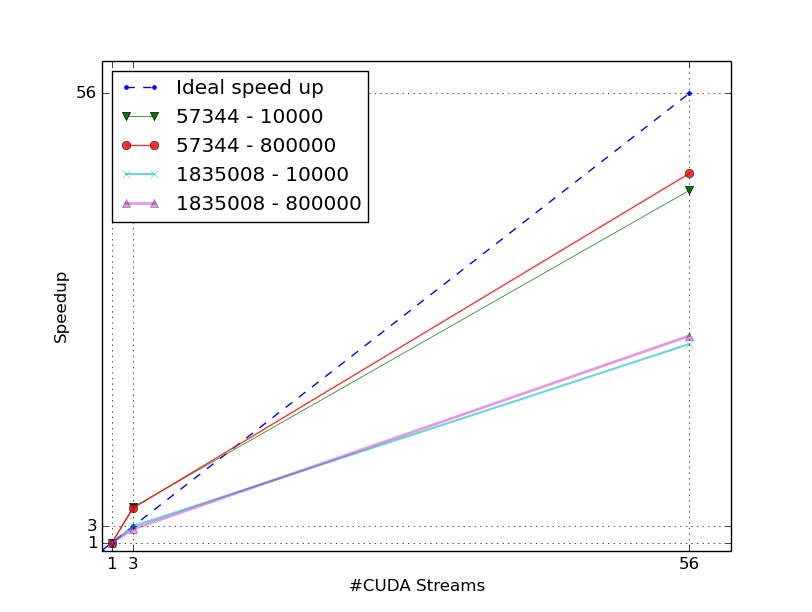
\includegraphics[scale=0.7]{plots/figure_25.png}
		\caption{Speedup for 3 and 56 CUDA streams on P100 device.}
		\label{fig:p100sp}
	%\end{figure}
	% \vspace*{\floatsep}
	%\begin{figure}
		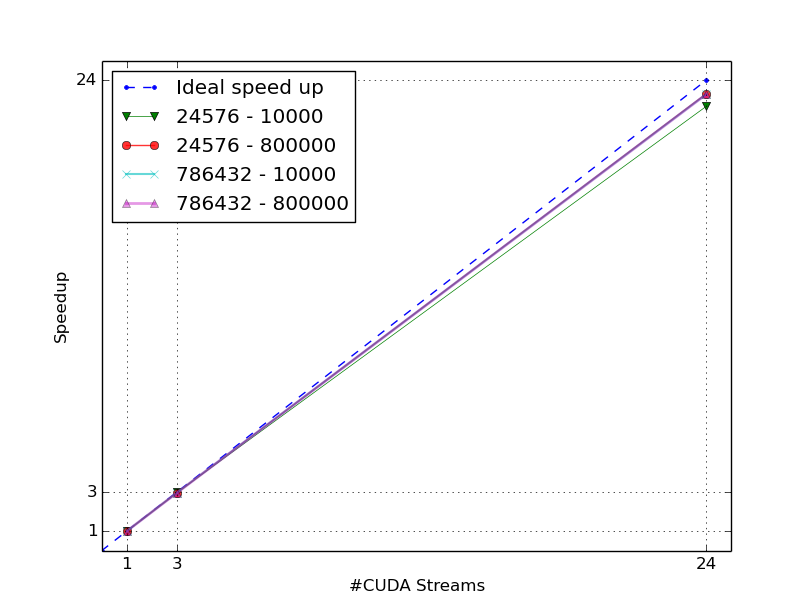
\includegraphics[scale=0.7]{plots/figure_26.png}
		\caption{Speedup for 3 and 56 CUDA streams on M40 device.}
		\label{fig:m40sp}
	\end{figure}
	To have an overall view on speedup we also present plots for both P100, in  \hyperref[fig:p100sp]{Figure 5.1}, and M40, in \hyperref[fig:m40sp]{Figure 5.2}.\\
	The two plots show the speedups only for a part of the real input dataset; in particular, each plot shows the smaller and bigger input stream length and for both it shows the smaller and bigger kernel iterations number.
	\begin{figure}
		\vspace{-2cm}
		\centering
		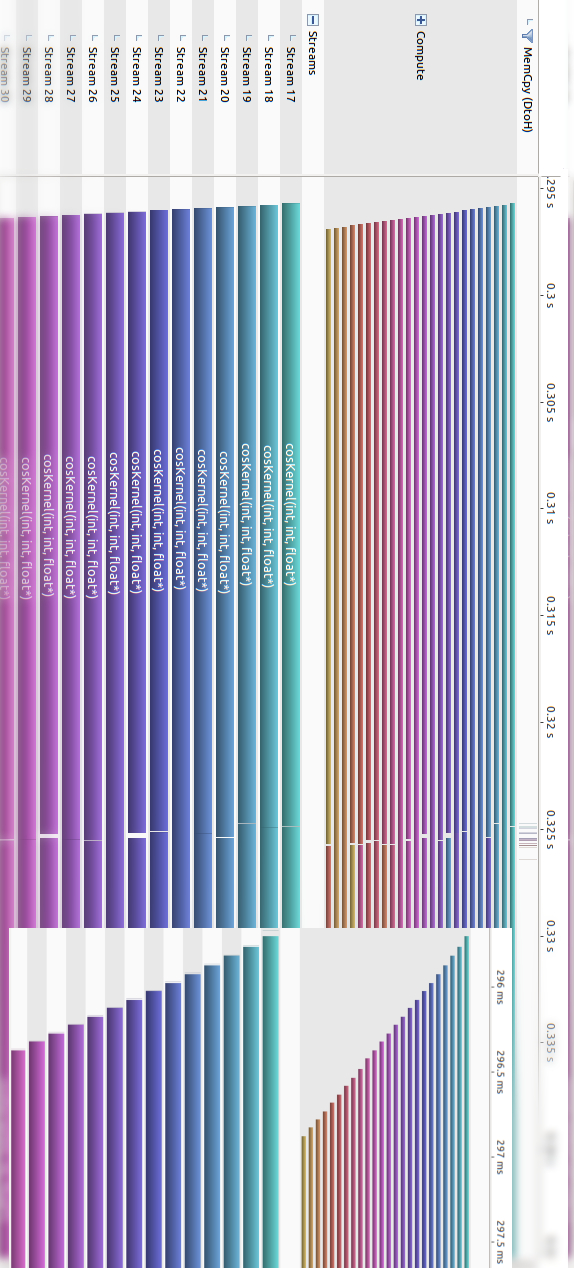
\includegraphics[scale=0.52]{plots/cos_profile.jpg}
		\caption{Profiling for an example execution: limit for input stream 786432, kernel iterations 10 000, 24 CUDA streams, on M40 device.}
		\label{fig:cosprofiling}
	
	\end{figure}
	
	From the two plots we can clearly see how performances increase proportionally with the number of CUDA streams\footnote{More precisely this gain is bounded to the number of Streaming Multiprocessors the GPU exploits.}.\\
	We can have a further proof of the achieved speedup, by running the \texttt{NVIDIA Visual Profiler}, we can see a portion of timeline representation in \hyperref[fig:cosprofiling]{Figure 5.3}. It's evident that we have a good overlapping between CUDA Streams, on the right side of the figure we can see a zoom in to the "\textit{stabilization phase}", ie the time interval it takes for the program to fill buffers and send them out to the device, until we reach a peak work rate and that "stairs" behavior vanishes.
	
	However the profiler analysis reported some issues in our code, for example the profiling showed a too much low grid/block size and a poor memory copy overlapping (having 2 data transfers at the same time). But all these issues are really dependent on the "extreme" use case we're approaching and, furthermore, they don't have a bad impact in this particular application.\\
	A good signal from the profiler is that the average usage of SMs, for a certain kernel call, is equal to one almost fully used SM. And this is exactly what we wanted to achieve, so this allows CUDA streams to spread kernel calls on all SMs, as soon as we have the maximum work rate.\\\\\\
	%BIGGER BUFFERS
	{\large \textbf{Bigger buffers}}\\\\
	As expected, we get about half the ideal speedup.\\
	This is because chunks of 2048 should take up the maximum possible for active threads per SM. This means having, for each kernel call, a grid containing 2 blocks, each of size 1024.\\
	So it seems that performances, in this kernel, are related to grid size. Recalling the smaller buffers, the profiler showed an almost full occupancy of one SM at \texttt{<<<1, 1024>>>} yet. So it makes sense to deduce that, \texttt{<<<2, 1024>>>} is a kernel configuration such that it occupies two SMs simultaneously. \\
	This is the same of having about the half of available resources.
	We show a plot about this result, tested on P100, in \hyperref[fig:biggerbufferspeedup]{Figure 5.4}
	
	\begin{figure}
		\vspace{-2cm}
		\centering
		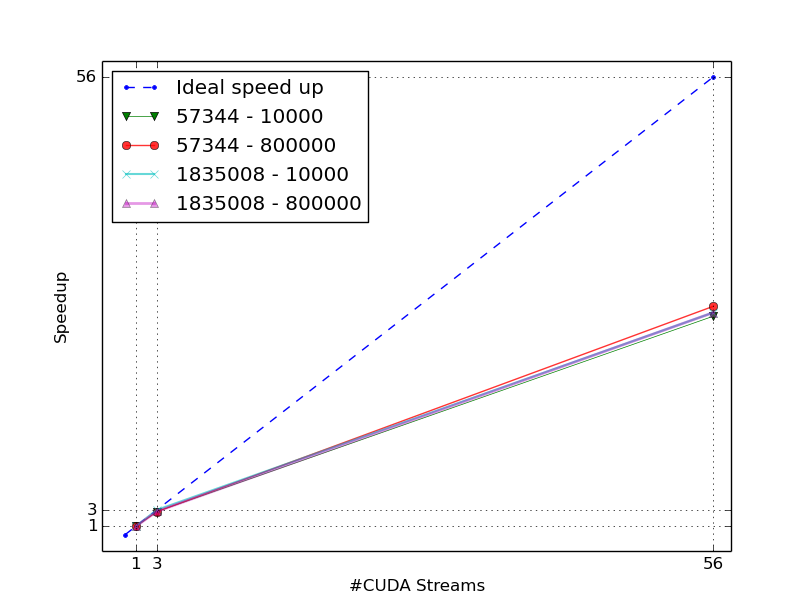
\includegraphics[scale=0.52]{plots/cos_speedup_biggerbuffer.png}
		\caption{Sublinear speedup in bigger buffers execution, the performances drop by a factor of 2.}
		\label{fig:biggerbufferspeedup}
		
	\end{figure}








%%%%%%%%%%%%%%%%%%%
%%%%% MAT MUL %%%%%
%%%%%%%%%%%%%%%%%%%
\section{Matrix Multiplication}
With Matrix multiplication we're facing a memory-bound kernel, so we had to make some slightly different tests with respect to the ones in simple-computation kernel.\\
Note that, even if the Farm logic is the same as the previous application, there are some details to redefine.\\
First of all, before we were dealing with an input stream of floats that were accumulated in buffers, here we have an \textit{input stream of matrices}. In particular as soon as we have two available input matrices (say \textit{A} and \textit{B}), they're sent out to device to apply the matrix multiplication kernel.\\
Finally we get back to host with the result matrix (say \textit{C}), that will be one of the output stream components.\\
For simplicity, we're measuring for square matrices case, even if code was implemented for non-square case too. 

Another assumption is that, for each Matrix Multiplication test, the kernel execution configuration was set up as follows:\\
assume \textit{N} to be the matrices order, then \texttt{BLOCK = 32} and
\texttt{GRID = (N/BLOCK) + BLOCK -1}, so we have:
\begin{center}	
	\texttt{blockSize = (BLOCK, BLOCK, 1)}\\
	\texttt{gridSize=(GRID, GRID, 1)}
\end{center}

We performed the following executions:
	\begin{table}	
		\centering
		\begin{tabular}{| c | c | c | c |} 
			\hline
			
			 \multicolumn{2}{c}{\textbf{Tesla P100}} & \multicolumn{2}{c}{\textbf{Tesla M40}} \\ [0.5ex]
			 % & \textbf{Tesla P100} & \textbf{Tesla M40} \\ 
			\hline
			
			\textbf{Mat. Order} & \textbf{In stream limit} & \textbf{Mat. Order} & \textbf{In stream limit}  \\ 
			\hline\hline
			128 & 225 & 64 & 100  \\ 
			\hline	
			256 & 441 & 128 & 196  \\ 
			\hline	
			512 & 900 & 256 & 400  \\ 
			\hline		
			1024 & 1764 & 512 & 784  \\ 
			\hline			
			2048 &  & 1024 &  \\
			\hline
			\hline				
			%3 670 016 & ---- & ---- & ---- \\
			%\hline
			
			\multicolumn{2}{c}{Data Parallel} &  \multicolumn{2}{c}{Data Parallel} \\ [0.5ex]
			% & \textbf{Data Parallel} & \textbf{Data Parallel} \\ 
			\hline\hline
			\multicolumn{2}{c}{1920} & \multicolumn{2}{c}{1280} \\ [0.5ex]
			% & \textbf{Data Parallel} & \textbf{Data Parallel} \\ 
			\hline			
			\multicolumn{2}{c}{2816} & \multicolumn{2}{c}{1792} \\ [0.5ex]
			\hline
			\multicolumn{2}{c}{3840} & \multicolumn{2}{c}{2560} \\ [0.5ex]
			\hline
			\multicolumn{2}{c}{5632} & \multicolumn{2}{c}{3584} \\ [0.5ex]
			\hline
			\multicolumn{2}{c}{7680} & \multicolumn{2}{c}{5120} \\ [0.5ex]
			\hline
			\multicolumn{2}{c}{11264} & \multicolumn{2}{c}{7168} \\ [0.5ex]
			\hline

		\end{tabular}
		\caption{Input dataset for Matrix Multiplication kernel. Above Stream parallel configuration, below Data Parallel correspondent.}	
		\label{tab:matdata}		
	\end{table}
	
\begin{enumerate}
	\item \textbf{Classic data parallel approach}
	Again, we have to put a limit on input stream, so that we can measure completion times. Note that the length limit for input, doesn't straightly correspond to the effective number of incoming matrices, but to the number of matrix multiplication that will be performed.\\
	So, say we have \( l\) as limit, it correspond to have \(2\cdot l\) matrices for input stream (A and B) and effectively \(l\) result matrices (C).
	
	To test the data parallel version it suffices to treat input/output streams as huge matrices (but we'll have only one matrix both for A,B and C).
	This means that we'll do computations, no longer on stream of small data structures, but on a unique big data structure.\\
	
	So, for example:
	\begin{itemize}
		\item We have two input streams, each has limit to 9 square matrices of order 2 (one input stream is for \textbf{A} matrices and one for \textbf{B});
		\item So suppose that our stream parallel model, sends out one matrix A and one B at time;
		\item Then we launch the kernel, performing the matrix multiplication, this will give back a matrix result C;
		\item This means in total we will perform 9 multiplications between couples of matrices, giving 9 result matrices;
		\item If we consider those 9 small matrices as block matrices, we can combine them into a bigger one;
		\item This will be equivalent to pick A and B matrices each of order 6;
		\item note that, for simplicity, we'll choose as input stream limit a square number, so that the equivalent combined data structure will be again square;
		\item In our example 9 is a square number so that we can obtain as composed matrix dimension \([(2\cdot3)\times(2\cdot3)] = [6\times6]\)  
	\end{itemize} 
	In \hyperref[tab:matdata]{Table 5.5}, in the lower portion, are showed the matrices orders we used to test data parallel version for matrix multiplication. 
	By giving these values as (square) matrix dimension and computing only one multiplication between matrices, we'll get the a balanced comparison to some Stream parallel versions.
	% \footnote{We'll see later what cases we match between data and stream parallel to make comparisons.}.
	
	\item \textbf{Streaming parallel}
	As we mentioned before, we have to put a limit on the stream length for both streams of input matrices.\\
	In the upper portion of \hyperref[tab:matdata]{Table 5.5} are reported all input stream limits and, for each of them, we test all of matrices order.\\
	For every combination given by the input dimensions, we'll test for different numbers of CUDA streams: \textbf{Zero}, \textbf{Three} and \textbf{N\textsubscript{SM}} CUDA Streams (with \(N_{SM} \ =\# Streaming \ Multiprocessors\)).
	The above test on different numbers of non-default streams, is implemented in a totally analogous way to the one for Simple-computation Kernel.
	% And the reasons why we test for those numbers of streams are the same too.
\end{enumerate}



\subsection{Results}
\begin{table}	
	\centering
	\begin{tabular}{ | c c c  || c c c | } 
		\hline
		\multicolumn{3}{c}{\textbf{Tesla P100 (zero Streams)}} & \multicolumn{3}{c}{\textbf{Tesla M40 (zero Streams)}}\\ [0.5ex]
		% & \textbf{Tesla P100} & \textbf{Tesla M40} \\ 
		\hline
		Event Times  & Number of Mats & Mat. Order & Event Times  & Number of Mats & Mat. Order  \\
		\hline\hline
		
		
		86.8854&	225&	\multirow{4}{*}{128}&	17.4869&	100&	\multirow{4}{*}{64}\\
		175.189&	441&	&	34.8778&	196&	\\
		359.9716&	900&	&	70.9718&	400&	\\
		725.5573&	1764&	&	139.3896&	784&	\\
		\hline
		334.0376&	225&	\multirow{4}{*}{256}&	36.2095&	100&	\multirow{4}{*}{128}\\
		672.9463&	441&	&	74.2685&	196&	\\
		1435&	900&	&	147.7336&	400&	\\
		2828.5366&	1764&	&	299.138&	784&	\\
		\hline
		1673.2133&	225&	\multirow{4}{*}{512}&	186.3913&	100&	\multirow{4}{*}{256}\\
		3325.6533&	441&	&	368.6813&	196&	\\
		6611.7566&	900&	&	786.7536&	400&	\\
		12919.6666&	1764&	&	1603.4933&	784& \\
		\hline
		10998.7666&	225&	\multirow{4}{*}{1024}&	1256.4&	100&	\multirow{4}{*}{512}\\
		21511.1666&	441&	&	2479.4333&	196&	\\
		43828.7666&	900&	&	5162.6333&	400&	\\
		85853.0333&	1764&	&	9791.98&	784&	\\
		\hline
		80764.8666&	225&	\multirow{4}{*}{2048}&	9075.22&	100&	\multirow{4}{*}{1024}\\
		158136.3333& 441&	&	17849.5666&	196&	\\
		309724.6666& 900&	&	36441.3666&	400&	\\
		604324&	1764&	&	72396.8666&	784&	\\
		
		\hline
		
	\end{tabular}
	\caption{Device completion times for Mat-Mul kernel, without using CUDA Streams (zero streams), results are reported for both P100 and M40.}	
	\label{tab:matvgszero}		
\end{table}

\begin{table}	
	\centering
	\begin{tabular}{ | c c c  || c c c | } 
		\hline
		\multicolumn{3}{c}{\textbf{Tesla P100 (3 Streams)}} & \multicolumn{3}{c}{\textbf{Tesla M40 (3 Streams)}}\\ [0.5ex]
		% & \textbf{Tesla P100} & \textbf{Tesla M40} \\ 
		\hline
		Event Times  & Number of Mats & Mat. Order & Event Times  & Number of Mats & Mat. Order  \\
		\hline\hline

		25.5549& 225&	\multirow{4}{*}{128}&	5.2046&	100&	\multirow{4}{*}{64}\\
		53.2203&	441&	&	10.7422&	196&	\\
		102.0575&	900&	&	23.9773&	400&	\\
		193.2436&	1764&	&	47.1808&	784&	\\
		\hline
		148.1446&	225&	\multirow{4}{*}{256}&	21.5294&	100&	\multirow{4}{*}{128}\\
		289.6773&	441&	&	41.9395&	196&	\\
		590.6776&	900&	&	74.5879&	400&	\\
		1157&	1764&	&	143.3123&	784&	\\
		\hline
		1173.3466&	225&	\multirow{4}{*}{512}&	129.985&	100&	\multirow{4}{*}{256}\\
		2298.3866&	441&	&	254.2516&	196&	\\
		4690.97&	900&	&	518.3303&	400&	\\
		9205.5&	1764&	&	1016.28&	784&	\\
		\hline
		9371.7766&	225&	\multirow{4}{*}{1024}&	1033.9166&	100&	\multirow{4}{*}{512}\\
		18371.2666&	441&	&	2027.17&	196&	\\
		37480.4&	900&	&	4136.54&	400&	\\
		73258.6666&	1764&	&	8113.0933&	784&	\\
		\hline
		74966.4666&	225&	\multirow{4}{*}{2048}&	8273.1066&	100&	\multirow{4}{*}{1024}\\
		146156.3333&	441&	&	16194.1&	196&	\\
		285788.3333&	900&	&	33041.1&	400&	\\
		559469.6666&	1764&	&	64763.6666&	784&	\\
		\hline
	\end{tabular}
	\caption{Device completion times for Mat-Mul kernel, with three CUDA Streams, results are reported for both P100 and M40.}	
	\label{tab:matvgsThree}		
\end{table}


\begin{table}	
	\centering
	\begin{tabular}{ | c c c  || c c c | } 
		\hline
		\multicolumn{3}{c}{\textbf{Tesla P100 (56 Streams)}} & \multicolumn{3}{c}{\textbf{Tesla M40 (24 Streams)}}\\ [0.5ex]
		% & \textbf{Tesla P100} & \textbf{Tesla M40} \\ 
		\hline
		Event Times  & Number of Mats & Mat. Order & Event Times  & Number of Mats & Mat. Order  \\
		\hline \hline
		20.8758&	225&	\multirow{4}{*}{128}&	2.739&	100&	\multirow{4}{*}{64}\\
		40.5783&	441&	&	5.0942&	196&	\\
		74.6636&	900&	&	10.0277&	400& \\
		145.4766&	1764&	&	19.8252&	784&	\\
		\hline
		147.765&	225& \multirow{4}{*}{256}&	19.3538&	100&	\multirow{4}{*}{128}\\
		288.5343&	441&	&	37.8560&	196&	\\
		588.9643&	900&	&	65.6809&	400&	\\
		1153.7333&	1764&	&	128.317&	784&	\\
		\hline
		1173.32&	225&\multirow{4}{*}{512}&	130.0533&	100&	\multirow{4}{*}{256}\\
		2298.3966&	441&	&	254.281&	196&	\\
		4690.9633&	900&	&	518.615&	400&	\\
		9202.3333&	1764&	&	1016.55&	784&	\\
		\hline
		9371.0433&	225&	\multirow{4}{*}{1024}&	1034.0666&	100&	\multirow{4}{*}{512}\\
		18374.7&	441&	&	2027.2866&	196&	\\
		37474.7&	900&	&	4136.7066&	400&	\\
		73348.3333&	1764&	&	8110.9966&	784&	\\
		\hline
		74971.6666&	225&	\multirow{4}{*}{2048}&	8262.7533&	100&	\multirow{4}{*}{1024}\\
		146175.6666&	441&	&	16202.4666&	196&	\\
		285955.6666&	900&	&	33059.2666&	400&	\\
		559425&	1764&	&	64786.5333&	784&	\\
		\hline
	\end{tabular}
	\caption{Device completion times for Mat-Mul kernel, with as many CUDA Streams as SM number, results are reported for both P100 and M40.}	
	\label{tab:matvgsSM}		
\end{table}

All the above tests, on Matrix Multiplication Kernel, give us the measures of device times.\\
Below we'll see that completion times and performance will notably be different, with respect to the previous computation-bound application.

All collected elapsed times are reported in \hyperref[tab:matvgszero]{Table 5.6}, for the zero-streams version, in \hyperref[tab:matvgsThree]{Table 5.7}, for the three-streams one, and \hyperref[tab:matvgsSM]{Table 5.8}, for the SM-streams version.\\
From these tables we can highlight some behaviors:
\begin{itemize}
	\item input streams of matrices have lengths that grow by a factor of 2 and it's easy to see that this makes a proportional increase in completion times, ie even measures grows by factors of 2;
	
	\item input matrix sizes again grow of \(2\times\) each, but in this case the completion times don't grow proportionally;
	
	\item for zero-streams we can see that, as the matrix order grows by a factor 2, the completion time can increase from \(\approx4\times\) to \(\approx7\times\); 
	
	\item for three-streams we can see that, as the matrix order grows by \(2\times\), the completion time can increase from \(\approx5\times\) to \(\approx8\times\); 
	
	\item finally for SM-streams we can see that, the completion time can increase from \(\approx7\times\) to \(\approx8\times\).
\end{itemize}
Those evidences holds for both machines measures and they give some hints on matrix multiplication nature.\\
The first point tells us that: the elapsed time to send/receive to/from the device, grows linearly with the number of matrices, so this input parameter would not affect performances. Especially, no matter the CUDA streams amount we decide to use, the increase by 2x of matrices quantity, will always give a growth of 2x in measures.\\
To have a visual comparison, we show plots for completion times in \hyperref[fig:matcompsize]{Figures 5.5 - 5.6}, where we can have a graphical view of the completion time variation, as the matrices order grows (respectively on M40 and P100. In \hyperref[fig:matcompnum]{Figures 5.7-5.8}, instead, we have similar plots, but for the time changing as the number of matrices increments.
\begin{figure}
	\centering
	\vspace{-2cm}
	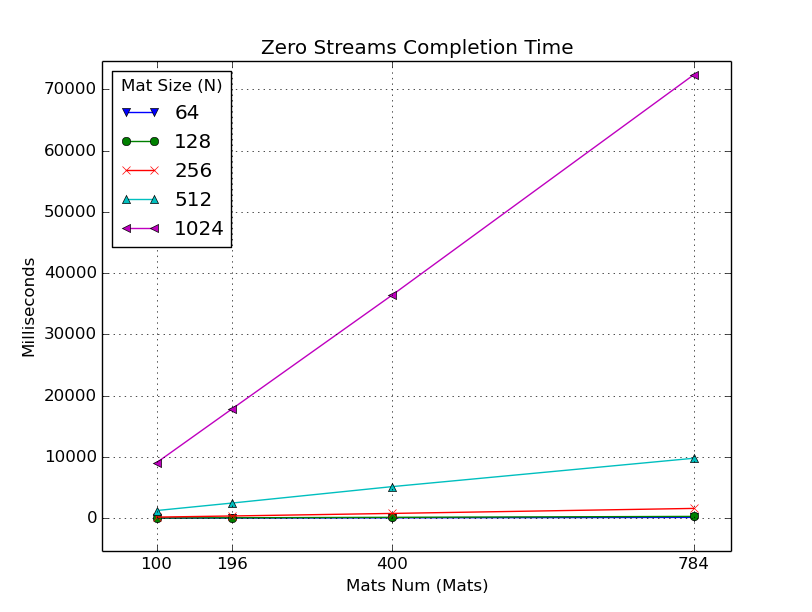
\includegraphics[scale=0.7]{plots/mat_comp_sizevar.png}
	\caption{Completion Time as the matrix order changes on M40.}
	
	%\end{figure}
	% \vspace*{\floatsep}
	%\begin{figure}
	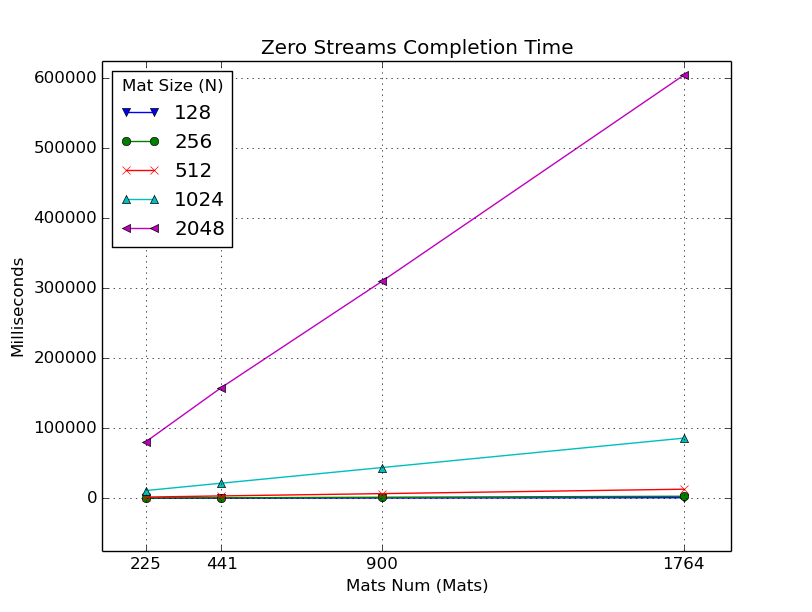
\includegraphics[scale=0.7]{plots/mat_comp_sizevar_P100.png}
	\caption{Completion Time as the matrix order changes on P100.}
	\label{fig:matcompsize}
\end{figure} 
\begin{figure}
	\centering
	\vspace{-2cm}
	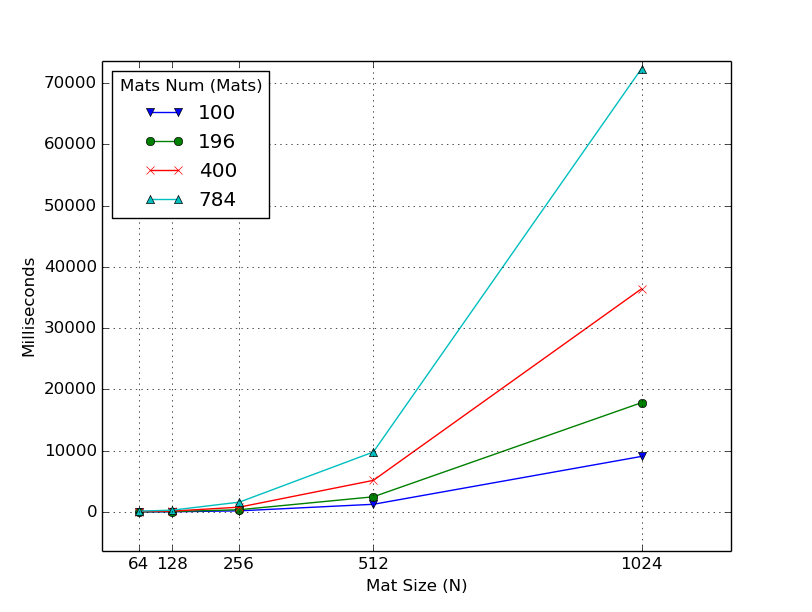
\includegraphics[scale=0.7]{plots/mat_comp_numvar.png}
	\caption{Completion Time as the number of matrices changes on M40.}
	
	%\end{figure}
	% \vspace*{\floatsep}
	%\begin{figure}
	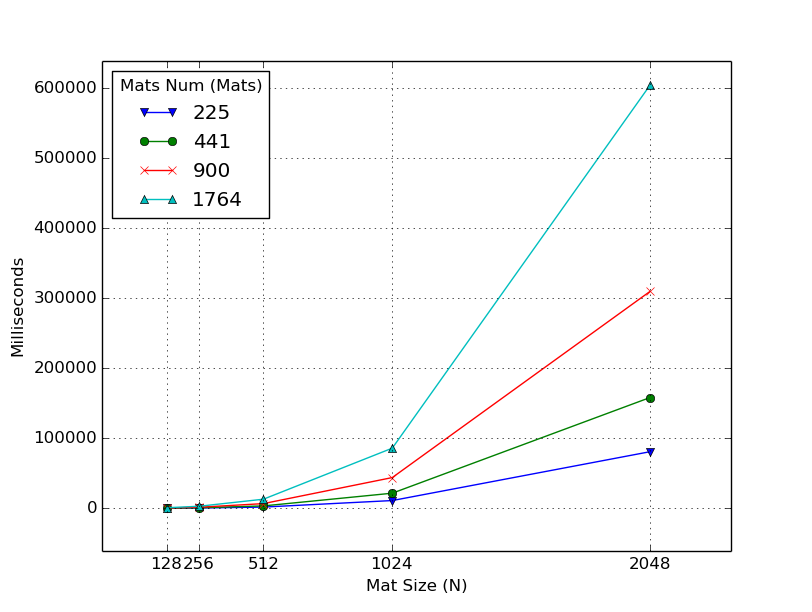
\includegraphics[scale=0.7]{plots/mat_comp_numvar_P100.png}
	\caption{Completion Time as the number of matrices changes on P100.}
	\label{fig:matcompnum}
\end{figure} 

The other points, emerging from completion times behavior, tell us that, as matrix order increases, we'll get worser and worser performances. Clearly this doesn't depend on CPU/GPU data transfers overhead, otherwise we'd have the same behavior when number of matrices grows.\\
So, the cause must reside on what happens inside the GPU. In reality, the classic matrix multiplication is a well known problem in GPUs paradigm and the classical implementation is known as a not efficient. \\
This is because, the simpler implementation, at each iteration, spends more time in \textit{global memory}/\textit{registers} transfers than in effective calculations. So that's why this kind of matrix multiplication is considered memory-bound.\\
So, the more elements a matrices have, the more data transfers (internal to the device) the GPU will have to perform and the more active threads will stall waiting for data to be available for computations.\\

\begin{table}	
	\centering
	\begin{tabular}{ | c | c | c | c  || c | c | c | c | } 
		\hline
		\multicolumn{4}{c}{\textbf{Tesla P100 (56 Streams)}} & \multicolumn{4}{c}{\textbf{Tesla M40 (24 Streams)}}\\ [0.5ex]
		% & \textbf{Tesla P100} & \textbf{Tesla M40} \\ 
		\hline
		\textbf{Mat. Number}  & \textbf{Mat. Order} & \textbf{Sp(3)} & \textbf{Sp(56)} & \textbf{Mat. Number}  & \textbf{Mat. Order}  & \textbf{Sp(3)} & \textbf{Sp(24)} \\
		\hline\hline
		
		
		225& \multirow{4}{*}{128}&	3.3999&	4.1620&	100&	\multirow{4}{*}{64}&	3.3598&	6.3839\\
		441& &	3.2917&	4.3173&	196&	&	3.2467&	6.8464\\
		900& &	3.5271&	4.8212&	400&	&	2.9599&	7.0775\\
		1764& &	3.7546&	4.9874&	784&	&	2.9543&	7.0309\\
		\hline
		225& \multirow{4}{*}{256}&	2.2548&	2.2606&	100& \multirow{4}{*}{128}& 1.6818&	1.8709\\
		441& & 2.3230&	2.3322&	196& & 1.7708& 1.9618\\
		900& & 2.4294&	2.4364&	400& & 1.9806&	2.2492\\
		1764& &	2.4447&	2.4516&	784& & 2.0873&	2.3312\\
		\hline
		225& \multirow{4}{*}{512}&	1.4260&	1.4260&	100& \multirow{4}{*}{256}&	1.4339&	1.4331\\
		441& &	1.4469&	1.4469&	196&  & 1.4500&	1.4498\\
		900& &	1.4094&	1.4094&	400& &	1.5178&	1.5170\\
		1764& &	1.4034&	1.4039&	784& &	1.5778&	1.5773\\
		\hline
		225& \multirow{4}{*}{1024}&	1.1736&	1.1736&	100&	\multirow{4}{*}{512}&	1.2151&	1.2150\\
		441& &	1.1709&	1.1706&	196& & 1.2231&	1.2230\\
		900& &	1.1693&	1.1695&	400& &	1.2480&	1.2480\\
		1764& &	1.1719&	1.1704&	784& &	1.2069&	1.2072\\
		\hline
		225& \multirow{4}{*}{2048}&	1.0773&	1.0772&	100&	\multirow{4}{*}{1024}&	1.0969&	1.0983\\
		441& &	1.0819&	1.0818&	196& &	1.1022&	1.1016\\
		900& &	1.0837&	1.0831&	400& &	1.1029&	1.1023\\
		1764& &	1.0801&	1.0802&	784& &	1.1178&	1.1174\\
		
		\hline
		
		
	\end{tabular}
	\caption{Here are showed speedups for all data sets of matrix multiplication kernel. Results are reported for both devices.}	
	\label{tab:matspeedup}		
\end{table}
So we'll now focus on speedups, to see that this memory-bound behavior will be reflected on GPU Farm approach. All speedups are listed in \hyperref[tab:matspeedup]{Table 5.9}.\\
From those results, we can mainly observe that:
\begin{itemize}
	\item \textit{Sp(3)} gives results near to the expected value, ie \(\approx 3\) for the smaller matrix sizes (128-256 for the P100, 64 for the M40);
	
	\item 	\textit{Sp(SM)} gives a really poor gain w.r.t. \textit{Sp(3)};
	
	\item all speedups degrade  to \(\approx1\) as the matrix order grows.
\end{itemize}

\begin{figure}[!tbp]
	\centering
	\vspace{-2cm}
	\hspace*{-1cm}
	\begin{tabular}[c]{ccc}
			
		\begin{tabular}{l}
			\subfloat[Matrix size 1024]{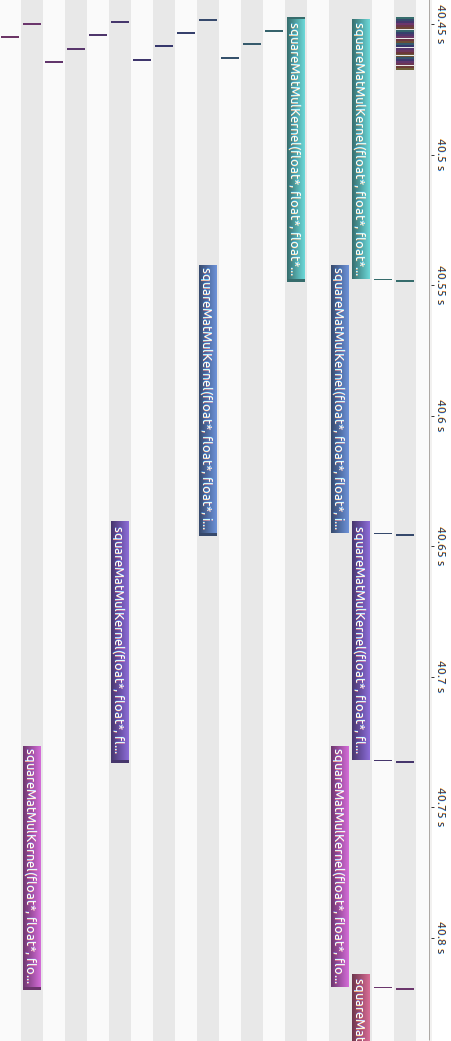
\includegraphics[width=0.32\textwidth]{plots/matmul784_1024_timeline.png}\label{fig:timeln1024}}
		\end{tabular}
		 &
		
		\begin{tabular}{l}
			\subfloat[Matrix size 256]{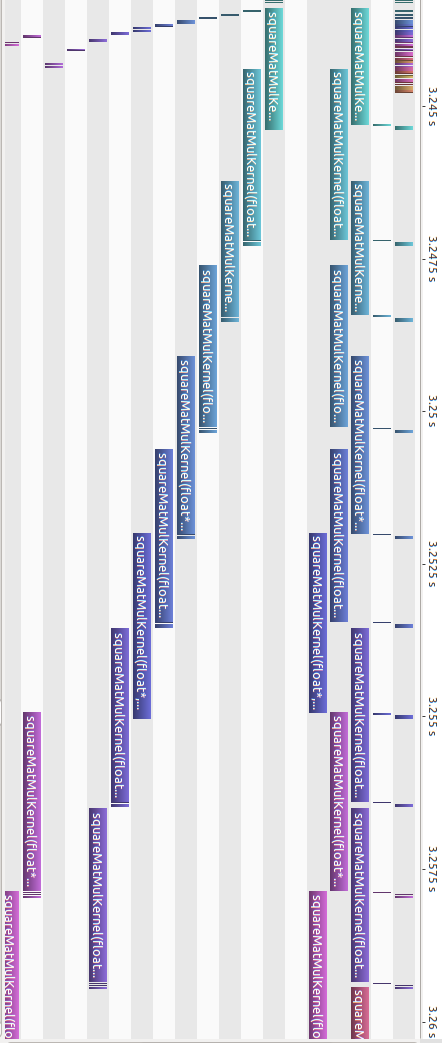
\includegraphics[width=0.32\textwidth]{plots/matmul784_256_timeline.png}\label{fig:timeln256}}
		\end{tabular} 
		& 
		\begin{tabular}{l}
		\subfloat[Matrix size 64]{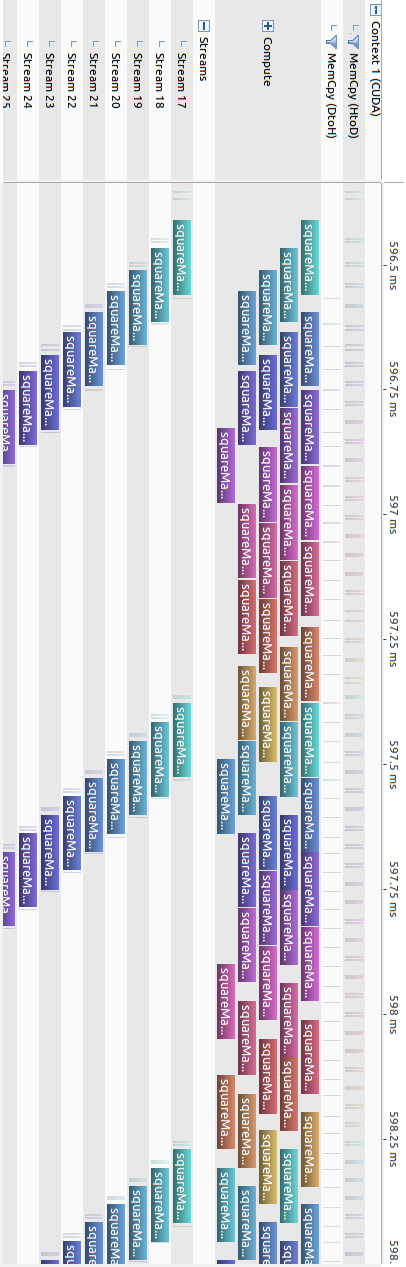
\includegraphics[width=0.45\textwidth]{plots/matmul784_64_timeline.png}\label{fig:timeln64}}
		\end{tabular}
		\\
	\end{tabular}    
	\caption{NVIDIA Visual profiler generated \textit{timeline} on M40, using 24 CUDA streams and running code for 784 matrices.}
	\label{fig:timeln}
\end{figure}

This behavior translates in the following: when the matrices get bigger, even if CUDA Streams push to have more simultaneous mat-mul, we'll have a lot of active threads (and so Multiprocessors) busy and probably mainly stalled on gathering floats from global memory.\\
This, in fact, inevitably leads to a very limited amount of gain, even when using a lot of CUDA streams. Furthermore, those results tells us that we will fit in Multiprocessor less matrix multiplication than we wish \footnote{Clearly this strictly holds for the type of matrix multiplication we implemented.}.\\
Furthermore, the necessity of having multiple blocks on grid, for this specific use case, translates in a monopolization of SMs resources by a small amount of kernel calls.\\

Profiling the application for some key data set we can inspect the above described facts and the relative reasons.

\begin{figure}[!tb]
	\centering
	\vspace{-2cm}
	%\hspace{2cm}
	\begin{tabular}[c]{cc}
		\multicolumn{2}{c}{\subfloat[Matrix size 64]{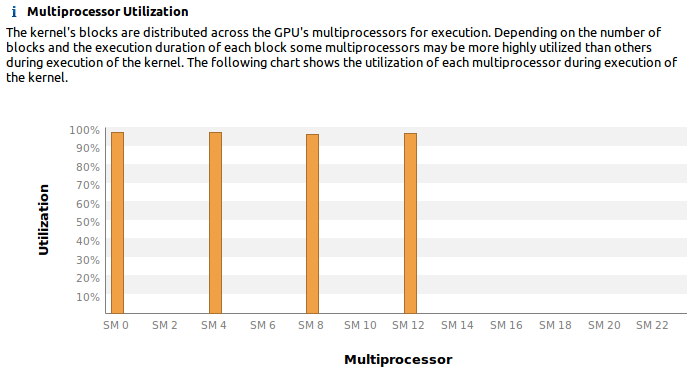
\includegraphics[width=\textwidth]{plots/matmul784_64_SMuse.png}\label{fig:SMuse64}}} \\
		
		\subfloat[Matrix size 1024]{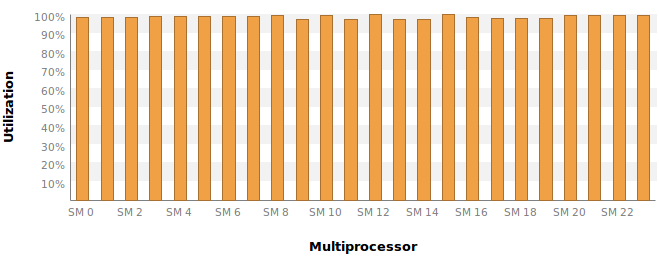
\includegraphics[width=0.5\textwidth]{plots/matmul784_1024_SMuse.png}\label{fig:SMuse1024}}
		&
		\subfloat[Matrix size 256]{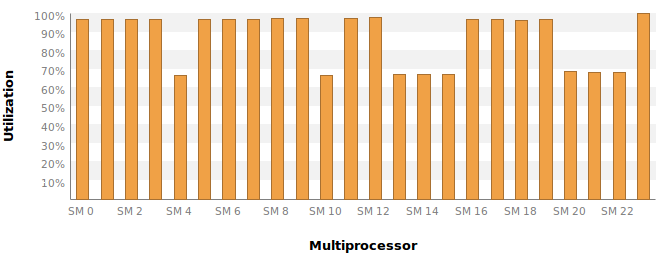
\includegraphics[width=0.5\textwidth]{plots/matmul784_256_SMuse.png}\label{fig:SMuse256}}\\

	\end{tabular}    
	\caption{NVIDIA Visual profiler generated \textit{timeline} on M40, using 24 CUDA streams and running code for 784 matrices.}
	\label{fig:SMuse}
\end{figure}

In \hyperref[fig:timeln]{Figure 5.9} we can have a visual cue on what is happening during an execution of mat-mul on M40, with 24 CUDA streams, having an input stream of 784 matrices of sizes: \(64\times64\) (\hyperref[fig:timeln64]{Figure 5.9 (c)}), \(256\times256\)(\hyperref[fig:timeln256]{Figure 5.9 (b)}), \(1024\times1024\)(\hyperref[fig:timeln1024]{Figure 5.9 (a)}).\\
Analyzing the figure we can see that the amount of overlapping, between operations in different streams, is quite limited in general, this just confirms what we saw from speedups.\\
From the above mentioned pictures, we can observe that in 64-sized case we're having a slightly better overlapping and a little more kernels running at the same time. In this case this may happens because grid and block sizes are smaller for each kernel launch, so this allow to have multiple kernels fit in SMs.

Having each thread block such that it contains \(32\times32\) threads, then a \(64\times64\) result matrix (say C) is managed by a grid of \(2\times2\) blocks, while a \(256\times256\) C is managed by a grid of \(8\times8\) blocks and, finally, a \(1024\times1024\) C is managed by a grid of \(32\times32\) blocks\footnote{This depends on how we implemented kernel launch, that is the classical kernel launch approach setting blocks at the maximum size possible. Remember implementations in \hyperref[chap:impl]{Chapter 4} and remember the kernel launch configuration explained above.}.\\
This means that, in the two latter cases, we don't even have all blocks, from a single kernel launch, fitting in all the SMs. If this may theoretically give a full occupancy of the GPU by a certain kernel, from the other side means saturate the cores without permitting other launches to fit, until the residing kernels ends or, at least, some resources are freed.

We can confirm this fact by looking at the occupancy graphs (generated from Visual Profiler), showed in \hyperref[fig:SMuse]{Figure 5.10}. In 64-sized case we've only 4 SMs almost fully employed, while in the other cases all SMs are almost busy (this holds on average in a single kernel launch).\\
The above cases exposes an example of the fact that \textit{not always a high or full occupancy may give better performances} \cite{loweroccupancy,cudabestpractices}, it strongly depends on the kernel nature.\\
On the other side as we decrease the matrices size we can't exploit enough resources. As we can see from \hyperref[fig:timeln64]{Figure 5.9} we have a better overlapping, but it seems that kernels lasts too little, so the host can't push kernels quickly enough to fill SMs. In fact Visual Profiler suggests us that those kernels perform a really poor amount of computations, especially with respect to memory latencies, see figure \hyperref[fig:mat62latency]{Figure 5.11}.\\ 
\begin{figure}[!tb]
	%\centering
	\vspace{-1cm}
	\hspace{-1cm}
	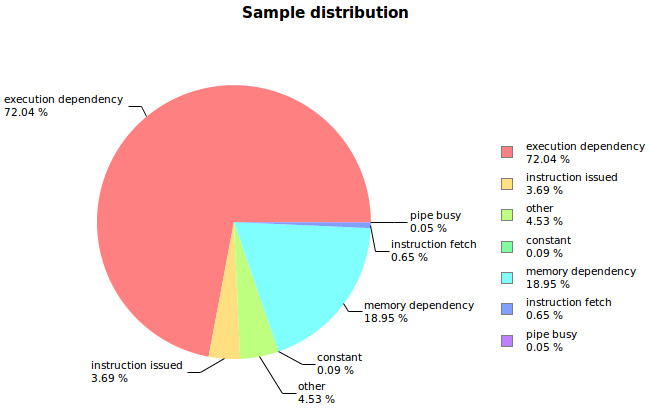
\includegraphics[scale=0.8]{plots/matmul784_64_kerlatencies.png}
	\caption{Nsight profiler execution on M40, 24 CUDA streams, 784 matrices of size 256. This graph gives the types and amounts of latencies inside mat-mul kernel execution.}
	\label{fig:mat62latency}
\end{figure}
This pie chart shows that most of the time kernels is idle on:
\begin{itemize}
	\item execution dependency\footnote{Execution dependency stall can be potentially reduced by increasing instruction-level parallelism Instruction-Level Parallelism (ILP), ie we can improve parallelism by increasing the amount of instructions for each thread. This can translate in less threads having a greater work-load each.}, ie an input required by the issued instruction isn't yet available; 
	
	\item memory dependency\footnote{ Memory dependency stall type can potentially be reduced by optimizing memory alignment and access patterns.}, a load/store cannot be made because the required resources aren't available or are fully utilized, or too many requests of a given type are outstanding.
\end{itemize}
This further demonstrates the fact that matrix multiplication is a memory-bound problem in GPU and, so, poor in computation amount.\\
This is why we have too much short kernels for smaller input data size and heavy kernels for bigger input sizes.


%%%%%%%%%%%%%%%%%%%%%%
%%%%% IMAGE PROC %%%%%
%%%%%%%%%%%%%%%%%%%%%%
\section{Image processing}
With image processing, ie Blur Box algorithm, we're facing a memory-bound kernel and especially rich of divergent execution flows, in fact we made similar tests to the ones for Matrix multiplication.\\
For each Image Processing test, the kernel execution configuration was set up as follows:\\
assume \textit{N} to be the image resolution (ie \(N\times N\), then \texttt{BLOCK = 1024} and
\texttt{GRID = (N/BLOCK) + BLOCK -1}, so we have:
\begin{center}	
	\texttt{blockSize = (BLOCK, 1, 1)}\\
	\texttt{gridSize=(GRID, 1, 1)}
\end{center}
Then we performed the following executions:
%BLOCK=1024
%imgSize=(128 256)
%#nStreams=(0 3 56)
%nImgs=(256 1024) # 14680064 29360128)
%dpSize=(4096 8192)


\begin{table}	
	\centering
	\begin{tabular}{| c | c |} 
		\hline
		
		 \multicolumn{2}{c}{\textbf{Tesla P100} \& \textbf{Tesla M40}} \\ [0.5ex]
		%& \textbf{Tesla P100} & \textbf{Tesla M40} \\ 
		\hline
		
		\textbf{Img. Order} & \textbf{In stream limit} \\ 
		\hline\hline
		128 & 64 \\ 
		\hline		
		256	& 256 \\ 
		\hline			
		512	& 1024 \\ 
		
		\hline\hline	
		\multicolumn{2}{c}{\textbf{Data Parallel Tesla P100 \& Tesla M40}} \\ [0.5ex] 
		
		\hline\hline		
		\multicolumn{2}{c}{1024 } \\ [0.5ex] 
		
		\multicolumn{2}{c}{2048 } \\ [0.5ex] 
		
		\multicolumn{2}{c}{4096 } \\ [0.5ex] 
		
		\multicolumn{2}{c}{8192 } \\ [0.5ex] 
		\hline	
	\end{tabular}
	\caption{Input dataset for Image Processing kernel. Above Stream parallel configuration, below the relative Data Parallel.}	
	\label{tab:imgdata}		
\end{table}

\begin{enumerate}
	\item \textbf{Classic data parallel approach}
	If we think to a picture as a matrix of pixels, then it's easy to see the analogy to the previous application.\\
	In particular the Data Parallel approach will be tested giving a single image of large dimensions, instead of a stream of small images.\\
	Again we're considering a single big image, as formed by merging smaller ones. Similarly to matrix multiplication case, we chose, as input stream limits, square numbers to make possible a balanced comparison to the correspondent square picture for data parallel.\\
	In the lower part of \hyperref[tab:imgdata]{Table 5.3} we show the order of dimension of the images used to compare to some streaming parallel cases.
	
	\item \textbf{Streaming parallel}
	
	As previous cases of Farm parallel pattern, we have to put a limit on the stream length for input stream of images.\\
	In the upper portion of \hyperref[tab:imgdata]{Table 5.10} are reported input stream limits and, for each of them, we test the three types of picture dimensions. Note that those images are square, so, for example, a size of 128 stands for a picture of \((128\times128)\) resolution (ie 16 384 pixels).\\
	For every combination given by the input dimensions, we'll test for different numbers of CUDA streams: \textbf{Zero}, \textbf{Three} and \textbf{N\textsubscript{SM}} CUDA Streams (with \(N_{SM} \ =\# Streaming \ Multiprocessors\)).
	The above test on different numbers of non-default streams, is implemented in a totally analogous way to the ones for the two applications showed above.
	
\end{enumerate}




\subsection{Results}
\begin{table}	
	\centering	
	\vspace*{-1cm}
	\begin{tabular}{ | c |  c c  || c | c | } 
		\hline

		CUDA Streams &	Img Number & Img Size & Tesla M40 & Tesla P100\\
		\hline\hline
		\multirow{8}{*}{0}&	64&	\multirow{2}{*}{128}&	1608.7367&	1425.9833\\
		&	256& &	6153.5800&	5670.5567\\
		&	1024& & 25422.7333&	22774.7333\\
		%\hline
		&	64&	\multirow{2}{*}{256}&	5099.54 &	4648.4467\\
		&	256&	&	20633.2 &	18077.1667\\
		&	1024&	&	81256 &	73411.1333\\
		%\hline
		&	64&	\multirow{2}{*}{512}&	15652.6333&	14281.8 \\
		&	256& &	63566.5333&	56694.1333\\
		&	1024& &	255928.3333&	224584.6667\\
		\hline
		\multirow{8}{*}{3}&	64&	\multirow{2}{*}{128}&	1547.5200&	963.1717\\
		&	256&	&	5477.0967&	3851.38\\
		&	1024&	&	21754.4667&	15387\\
		%\hline
		&	64&	\multirow{2}{*}{256}&	4557.1400&	3933.31\\
		&	256&	&	17582.4&	15724.8\\
		&	1024&	&	71291.5&	60029.0667\\
		%\hline
		&	64&	\multirow{2}{*}{512}&	14315.9333&	11833.2\\
		&	256&	&	56507.8667&	49691.8\\
		&	1024&	&	224832.3333&	197940.3333\\
		\hline
		\multirow{8}{*}{24 - 56}&	64&	\multirow{2}{*}{128}&	1482.0533&	1043.4733\\
		&	256&	&	5651.3833&	4178.6333\\
		&	1024&	&	21790.8333&	16213.8667\\
		&	64&	\multirow{2}{*}{256}&	4461.85&	3766.4833\\
		&	256&	&	17751.7667&	15682.6667\\
		&	1024&	&	70421.1&	63726.1667\\
		&	64&	\multirow{2}{*}{512}&	13900.0333&	12902.0667\\
		&	256&	&	54006.6667&	51737.7333\\
		&	1024&	&	226638&	208308.3333\\	
		\hline	
	\end{tabular}
	\caption{Device completion times for Image processing kernel, all types of tested CUDA Streams number are reported, results are given for both P100 and M40.}	
	\label{tab:imgavgs}		
\end{table}

As expected this image processing kernel demonstrates a bad fitting for Farm parallel pattern in GPU. It gives even worst performances than matrix multiplication.

We report in \hyperref[tab:imgavgs]{Table 5.11} all completion times, for zero-streams, three-streams and SM-streams versions.\\
We can see that the input stream of images grows in length by a factor 4, in fact completion times follow this trend by increasing \(\approx4\times\) proportionally with input limits.\\
Instead, fixed a certain number of images as input stream limit, the image size grows by a factor 2. This time this lead to an increasing of completion times by a slightly bigger factor, ie \(\approx3\times\).


\begin{table}	
	\centering
	\begin{tabular}{ | c  c || c | c  || c | c || } 
		\hline
		& &  \multicolumn{2}{c}{\textbf{Tesla M40 (24 Streams)}}& \multicolumn{2}{c}{\textbf{Tesla P100 (56 Streams)}} \\ [0.5ex]
		% & \textbf{Tesla P100} & \textbf{Tesla M40} \\ 
		\hline		
		Img Number &	Img Size&	\textbf{Sp(3)} & \textbf{Sp(24)} &	\textbf{Sp(3)} &	\textbf{Sp(56)}\\
		\hline	\hline	
		64&	\multirow{2}{*}{128}&	1.0396&	1.0855&	1.4805&	1.3666\\
		256&	&	1.1235&	1.0889&	1.4723&	1.3570\\
		1024&	&	1.1686&	1.1667&	1.4801&	1.4046\\
		64&	\multirow{2}{*}{256}&	1.1190&	1.1429&	1.1818&	1.2342\\
		256&	&	1.1735&	1.1623&	1.1496&	1.1527\\
		1024&	&	1.1398&	1.1539&	1.2229&	1.1520\\
		64&	\multirow{2}{*}{512}&	1.0934&	1.1261&	1.2069&	1.1069\\
		256&	&	1.1249&	1.1770&	1.1409&	1.0958\\
		1024&	&	1.1383&	1.1292&	1.1346&	1.0781\\
		\hline
	\end{tabular}
	\caption{Here are showed speedups for all data sets of image processing kernel. Results are reported for both devices.}	
	\label{tab:imgspeedup}		
\end{table}


But the really evident and important behavior is that we don't have much difference between the version not using CUDA Streams and the ones using them.\\
This is, in fact, confirmed by the speedups in \hyperref[tab:imgspeedup]{Table 5.12}, where we can see that almost everywhere the best speedup we can achieve is about 1.\\
This means that we almost have no overlapping, we expected a similar behavior though.\\




\section{Results Summary}
%Results are collected, for each group of execution, in some \texttt{.txt} files. In those files we can find a list of applications outputs in \texttt{.csv} format.
Merging all results we obtained, we can state that, under specific assumptions and adjustments, \textit{Farm parallel pattern can give a speedup really near to linear}.\\
We can observe this behavior especially in computational-bound case, where we're above the ideal speedup for a small quantity. We can't achieve perfectly the ideal for more possible reasons: 
\begin{itemize}
	\item First we've to take into account that we have a "\textit{stabilization phase}", meaning that when input stream starts to send first items we've a little interval where buffers need to fill up, until we reach the peak occupation for CUDA streams and so for SMs;
	\item We can have the rare situation where in a certain portion of time, say \([t_{i},t_{i}+\Delta_{t}\), we have multiple requests (from different CUDA Streams) for memory copy, ie we've \(>\#Copy Engines (=2)\) simultaneous requests.\\
\end{itemize}
However, we only proved theoretically that \(Sp_{\#SM} \leq \#SM\), just for completeness we could show some tests for a greater number of CUDA Streams, for example\\ \(\#CUDA Streams \geq 2\cdot\#SM\).
We briefly show the result for Simple-computational kernel, comparing the SM-version and the double-SM-version\footnote{We only report results for M40 machine, but performances are analogous on P100.}:



\begin{table}	
	\centering
	\begin{tabular}{ | c  c || c | c | } 
		\hline
		  N items & M iterations & Comp.Time (48 Streams) & Sp(48) \\ [0.5ex]
		% & \textbf{Tesla P100} & \textbf{Tesla M40} \\ 
		\hline	
		\hline	
	
		\multirow{2}{*}{245}&	10000&	35.6340&	19.4686\\
		& 	400000&	1204.41&	22.7945\\
		&	800000&	2379.3233&	23.0691\\
		\hline
		\multirow{2}{*}{49152}&	10000&	70.2144&	19.6877\\
		&	400000&	2380.3433&	23.0645\\
		&	800000&	4734.9566&	23.1857\\
		\hline
		\multirow{2}{*}{98304}&	10000&	135.2063&	20.4526\\
		&	400000&	4741.3866&	23.1576\\
		&	800000&	9537.72&	23.0194\\
		\hline
		\multirow{2}{*}{196608}&	10000&	282.214&	19.5913\\
		&	400000&	9893.6566&	22.1949\\
		&	800000&	19760.9333&	22.2204\\
		\hline
		\multirow{2}{*}{393216}&	10000&	519.2003&	21.2989\\
		&	400000&	18951.0666&	23.1750\\
		&	800000&	38050.7333&	23.0795\\
		\hline
		\multirow{2}{*}{786432}&	10000&	969.7603&	22.8021\\
		&	400000&	37473.3333&	23.4415\\
		&	800000&	74944.7333&	23.4355\\

		
		\hline
		
		
	\end{tabular}
	\caption{Here are showed completion time and speedup for \(48 = 2 \cdot \#SM\) CUDA Streams. }	
	\label{tab:cosdoublestream}		
\end{table}


And, as we expected, the \hyperref[tab:cosdoublestream]{Table 5.13} confirms the theoretical upper bound determined with Amdahl's law. The table clearly shows that the speedup is still \(Sp_{\#SM}\leq\#SM\).





\subsection{Stream parallel compared to Data parallel}
As introduced on the tests settings, we executed and collected completion time measures for data parallel version too.\\
The latter clearly is setup in such a way that it computes the same workload that we're computing in stream version.\\
Below we'll show results for each kernel type:
\begin{itemize}
	\item \textbf{Simple-computation kernel}\\%Dire che smaller buffer meglio perché non monopolizza interamente un SM, lascia spazio ad un altro kernel launch di entrare.
		
	\begin{table}
		\centering
		\begin{tabular}{ | c  c || c | c  || c | c || } 
			\hline
			& &  \multicolumn{2}{c}{\textbf{Tesla P100 (56 Streams)}}& \multicolumn{2}{c}{\textbf{Tesla M40 (24 Streams)}} \\ [0.5ex]
			% & \textbf{Tesla P100} & \textbf{Tesla M40} \\ 
			\hline		
			N items &	M iterations &	56 Streams & Data Parallel &	24 Streams & Data Parallel\\
			\hline	\hline	
			
			\multirow{2}{*}{57344}&	10000&	104.7727&	51.3901&	30.6074&	34.9234\\
			&	400000&	3968.9133&	1825.36&	1178.72&	1178.71\\
			&	800000&	7818.8433&	3648.6333&	2355.4133&	2352.63\\
			\hline
			\multirow{2}{*}{114688}&	10000&	205.7297&	90.2111&	60.2087&	58.0608\\
			&	400000&	7828.1933&	3574.74&	2358.6567&	2303.43\\
			&	800000&	15691.8333&	7145.6633&	4714.36&	4601.0867\\
			\hline
			\multirow{2}{*}{229376}&	10000&	407.712&	179.2643&	119.3447&	112.1287\\
			&	400000&	15687.9667&	7124.46&	4715.1233&	4456.6633\\
			&	800000&	31396&	24437.4333&	9425.92&	8910.3567\\
			\hline
			\multirow{2}{*}{458752}&	10000&	803.2237&	669.5133&	238.249&	241.901\\
			&	400000&	31422.0333&	26757.7&	9429.89&	9627.5267\\
			&	800000&	62818.7&	52896.3667&	18853.9667&	19256.4333\\
			\hline
			\multirow{2}{*}{917504}&	10000&	1619.5867&	1361.9133&	475.5907&	441.5377\\
			&	400000&	62793.4&	53258.9667&	18856.8&	17591.4667\\
			&	800000&	125575&	105657&	37705.6667&	35190.9\\
			\hline
			\multirow{2}{*}{1835008}&	10000&	3229.0633&	2682.6767&	949.497&	884.6433\\
			&	400000&	125547.6667&	105891&	37711.9&	35013.4667\\
			&	800000&	251503&	209018.6667&	75445.2667&	70397.2\\

			\hline

		\end{tabular}
		\caption{Simple-computational kernel. Comparison between completion times for stream parallel (max stream -56 and 24 respectively-) and data parallel versions. Results are reported for both devices.}	
		\label{tab:cosdataparVSsm}		
	\end{table}
	
	From the \hyperref[tab:cosdataparVSsm]{Table 5.14} we can clearly see that data parallel has really similar performances with respect to stream parallel (in SM-CUDA-streams setting).\\
	This is what we expected, since, the almost-linear speedup we obtained, means that we successfully overlapped different executions for small chunks. Formally, suppose to consider the amount of input data already splitted in \(k\) parts and suppose data parallel version's device completion time is give by the following formula:
	\begin{center}
		\(T_{DP} \approx k\cdot T_{items}\)
	\end{center}
	where \(T_{items}\) is the time needed to compute one of the \(k\) portions of data.
	% and \(T_{DPov}\) is the overhead given by data transfers (in data parallel we've only one to device and one from device).\\
	For stream parallel version we'll have instead
	\begin{center}
		\(T_{SP} \approx \Delta_{t} + \frac{k}{\#SM}\cdot T_{items}\)
	\end{center}
	where \(\Delta_{t}\) is a not predictable overhead, given by the temporal difference \(t_{r}- t_{0}\), \(t_{0}\) is when initially  the first item is sent for the first CUDA stream.\\
	 While \(t_{r}\) is the moment when the first element arrives for the \(r - th\) stream.\\
	In this \(\Delta_{t}\) we may also think to include other overheads due to small amount of time in which we have an imperfect streams overlapping. So, assuming \(\Delta_{t}\) to be negligible with respect to the time spent in computations, we can conclude:
	\begin{center}
		\(T_{DP} \approx k\cdot T_{items} \leq \Delta_{t} + \frac{k}{\#SM}\cdot T_{items}\approx T_{SP} \ \Rightarrow T_{DP} \  \approx T_{SP}\)
	\end{center}
	
	\item \textbf{Matrix Multiplication kernel}\\
	%	Dire che in sostanza si è capit oche per questo kernel e in versione Farm ci vuole un compromesso tra matrici grandi, quindi tanti blocchi, che saturano la GPU e matrici troppo piccole t.c il kernel dura troppo poco.
	In \hyperref[tab:matdataparVSsmM40]{M40 Table} and \hyperref[tab:matdataparVSsmP100]{P100 Table} we'll se a really particular behavior, because on both devices we get consistently better performances from streaming parallel version, with respect to the data parallel version.\\
	\begin{table}[!h]	
		\centering
		\begin{tabular}{ | c  c || c | c  || c || } 
			\hline
	 
		
			Mat Number&	Mat Order&	56 Streams&	Event Time&	Data Par Mat Order\\
			\hline	\hline	
			225&	\multirow{3}{*}{128}&	20.8758	& 289.4027&	1920\\
			441	& &	40.5783&	898.0440&	2688\\
			900	& &	74.6636&	2256.0733&	3840\\
			1764& &	145.4767&	7063.8233&	5376\\
			\hline
			225&	\multirow{3}{*}{256}&	147.7650&	2256.0733&	3840\\
			441	& &	288.5343&	7063.8233&	5376\\
			900	& &	588.9643&	17878.3667&	7680\\
			1764& &	1153.7333&	56190.3667&	10752\\
			\hline
			225&	\multirow{1}{*}{512}&	1173.3200&	17878.3667&	7680\\
			441	& &	2298.3967&	56190.3667&	10752\\
			\hline
		\end{tabular}
		\caption{Matrix multiplication kernel. Comparison between completion times for stream parallel (max stream -56) and data parallel versions (Partial dataset is of stream version is considered). Results are reported for P100.}	
		\label{tab:matdataparVSsmP100}		
	\end{table}
	
	For Completeness in \hyperref[tab:matdataparVSsmM40]{M40 Table} we also introduced a column to compare the data parallel version with serial version (streaming parallel with zero CUDA Streams).\\
	From that column we can see that Data parallel version also has worse performances than serial version. Furthermore we introduced a column to compute the ratio \(T_{dataParallel} \ T_{\#SM streams}\), and as we can see that from Stream Parallel version we have a gain of \(\approx 20\times\).
	
	\begin{table}[!h]
		\centering
		\begin{tabular}{ | c  c || c | c  || c | c | c  || } 
			\hline
		
		\makecell{	Mat\\ Number}&	\makecell{Mat\\ Order}&	Zero Streams&	24 Streams&	Data Parallel& \makecell{Mat Order\\Data Par}&	(DataPar)/(24Str)\\
			\hline	\hline	
			100&	\multirow{3}{*}{128}&	36.2095&	19.3538&	172.6997&	1280&	8.9233\\
			196	& &	74.2686&	37.8561&	456.3713&	1792&	12.0554\\
			400	& &	147.7337&	65.6809&	1315.6467&	2560&	20.0309\\
			784	& &	299.1380&	128.3170&	3590.4367&	3584&	27.9810\\
			\hline
			100&	\multirow{3}{*}{256}& 186.3913&	130.0533& 1315.6467&	2560& 10.1162\\
			196& &	368.6813&	254.2810&	3590.4367&	3584&	14.1200\\
			400	& &	786.7537&	518.6150&	10437.7&	5120&	20.1261\\
			784	& &	1603.4933&	1016.55&	28711&	7168&	28.2436\\
			\hline
			100&	\multirow{1}{*}{512}&	1256.4&	1034.0667&	10437.7&	5120&	10.0938\\
			196& &	2479.4333&	2027.2867&	28711&	7168&	14.1623\\
		\hline
		\end{tabular}
		\caption{Matrix multiplication kernel. Comparison between completion times for stream parallel (max stream -24-) and data parallel versions (Partial dataset is of stream version is considered). Results are reported for M40.}	
		\label{tab:matdataparVSsmM40}		
	\end{table}
	This singular behavior again depends on the memory-bound nature of this implementation.\\
	Having a huge data structure, computing simple operations on a huge amount of items residing in global memory, inevitably leads to a over-occupancy in SMs (mainly due to latencies and thread stalls), dropping dramatically performances.
	
	
	\item \textbf{Image Processing kernel}\\
	In this case, looking at \hyperref[tab:imgdataparVSsm]{Table 5.17}, we can observe a fluctuation in behavior.\\
	Sometimes Data Parallel performs better than Stream Parallel, and sometimes the vice versa happens. But we recall that this type of kernel is peculiarly chosen to have divergent flows. Indeed, even the profiler reported as an issue the latency due to diverging flows.
	\begin{table}
		\centering
		\begin{tabular}{ | c  c || c | c  || c | c || c|| } 
			\hline
			& &  \multicolumn{2}{c}{\textbf{Tesla M40 (24 Streams)}}& \multicolumn{2}{c}{\textbf{Tesla P100 (56 Streams)}}& \\ [0.5ex]
			% & \textbf{Tesla P100} & \textbf{Tesla M40} \\ 
			%\hline		
			%Img Number &	Img Size&	\textbf{Sp(3)} & \textbf{Sp(24)} &	\textbf{Sp(3)} &	\textbf{Sp(56)}\\
			\hline							M40	
			Img Number&	Img Size&	Streams 56&	Data Par&	Streams 24&	Data Par	& Img Size\\
			\hline	\hline	
			64&	\multirow{2}{*}{128}&	1043.4733&	1042.1233&	1482.0533&	1928.8767&	1024\\
			256	& &	4178.6333&	2522.0767&	5651.3833&	7369.49&	2048\\
			1024& &	16213.8667&	25430.7667&	21790.8333&	29222.2&	4096\\
			\hline	
			64&	\multirow{1}{*}{256} & 3766.4833 & 2522.0767 & 4461.85&	7369.49&	2048\\
			256	& &	15682.6667&	25430.7667&	17751.7667&	29222.2&	4096\\
			1024 & & 63726.1667&	46776.4667&	70421.1&	50971.8333&	8192\\
			\hline	
			64&	\multirow{1}{*}{512} & 12902.0667 & 25430.7667&	13900.0333 & 29222.2 & 4096\\
			256& &	51737.7333&	46776.4667&	54006.6667&	50971.8333&	8192\\
			
		\hline			
		\end{tabular}
		\caption{Here is showed the data parallel vs. stream parallel comparison for image processing kernel. Results are reported for both devices.}	
		\label{tab:imgdataparVSsm}		
	\end{table}
	
	
\end{itemize}


